\ifx\allfiles\undefined
\documentclass[8pt a4paper, oneside, UTF8]{ctexbook}  % +  这一句是新增加的
\usepackage{amsmath}   % 数学公式
\usepackage[dvipsnames]{xcolor}
\usepackage{amsthm}    % 定理环境
\usepackage{amssymb}   % 更多公式符号
\usepackage{graphicx}  % 插图
\usepackage{mathrsfs}  % 数学字体
\usepackage{enumitem}  % 列表
\usepackage{geometry}  % 页面调整
\usepackage{unicode-math}
\usepackage{extarrows}
\usepackage{subfigure}
\usepackage{extarrows}
\usepackage{footnote}
\usepackage{svg}
\usepackage[colorlinks,linkcolor=black]{hyperref}
\usepackage{supertabular}
\usepackage{tcolorbox}
\usepackage{ulem}
\usepackage{framed}
\usepackage{float}
\usepackage{microtype}
\newcommand{\arccot}{\mathrm{arccot}\,}
\tcbuselibrary{breakable}
\tcbuselibrary{most}
\newcounter{problemname}
\newenvironment{solution}{\par\noindent\textbf{解答. }}{\par}
\newenvironment{note}{\par\noindent\textbf{题目\arabic{problemname}的注记. }}{\par}
\definecolor{shadecolor}{RGB}{241, 241, 255}
\newenvironment{problem}{\begin{shaded}\stepcounter{problemname}\par\noindent\textbf{题目\arabic{problemname}. }}{\end{shaded}\par}

\graphicspath{ {figure/},{../figure/}, {config/}, {../config/} }  % 配置图形文件检索目录
\linespread{1.2} % 行高

% 页码设置
\geometry{top=25.4mm,bottom=25.4mm,left=20mm,right=20mm,headheight=2.17cm,headsep=4mm,footskip=12mm}

% 设置列表环境的上下间距
\setenumerate[1]{itemsep=5pt,partopsep=0pt,parsep=\parskip,topsep=5pt}
\setitemize[1]{itemsep=5pt,partopsep=0pt,parsep=\parskip,topsep=5pt}
\setdescription{itemsep=5pt,partopsep=0pt,parsep=\parskip,topsep=5pt}

% 定理环境
% ########## 定理环境 start ####################################

% #### 将 config.tex 中的定理环境的对应部分替换为如下内容
% 定义单独编号,其他四个共用一个编号计数 这里只列举了五种,其他可类似定义(未定义的使用原来的也可)
\newtcbtheorem[auto counter, number within=section, list type=subsubsection, list inside=toc]{defn}{定义}
{
    colback=green!5,colframe=green!35!black,fonttitle=\bfseries, title={Comment \thetcbcounter}, list entry={Comment \thetcbcounter\quad}, %标题
    breakable, %支持跨页
    before upper={\parindent10pt\noindent},  % 支持缩进。\noindent:首行不缩进
    % left = 2mm, %文字离线框左边的边距
    % right = 1mm,%同上
    % top = 1mm,%同上
    % bottom = 1mm,%同上
    % arc is angular = 1mm, % 棱角线框
    % sharp corners, % 直角线框
    % enhanced,frame hidden, % 隐藏线框
    % enhanced, drop fuzzy shadow,  % 显示阴影
}
{def}

\newtcbtheorem[auto counter, number within=section, list type=subsubsection, list inside=toc]{lemma}{引理}
{
    colback=SeaGreen!10!CornflowerBlue!10,colframe=RoyalPurple!55!Aquamarine!100!,fonttitle=\bfseries, title={Comment \thetcbcounter}, list entry={Comment \thetcbcounter\quad}, %标题
    breakable, %支持跨页
    before upper={\parindent10pt\noindent},  % 支持缩进。\noindent:首行不缩进
    % left = 2mm, %文字离线框左边的边距
    % right = 1mm,%同上
    % top = 1mm,%同上
    % bottom = 1mm,%同上
    % arc is angular = 1mm, % 棱角线框
    % sharp corners, % 直角线框
    % enhanced,frame hidden, % 隐藏线框
    % enhanced, drop fuzzy shadow,  % 显示阴影
}
{lem}


\newtcbtheorem[auto counter, number within=section, list type=subsubsection, list inside=toc]{them}{定理}
{
    colback=Salmon!20, colframe=Salmon!90!Black,fonttitle=\bfseries, title={Comment \thetcbcounter}, list entry={Comment \thetcbcounter\quad}, %标题
    breakable, %支持跨页
    before upper={\parindent10pt\noindent},  % 支持缩进。\noindent:首行不缩进
    % left = 2mm, %文字离线框左边的边距
    % right = 1mm,%同上
    % top = 1mm,%同上
    % bottom = 1mm,%同上
    % arc is angular = 1mm, % 棱角线框
    % sharp corners, % 直角线框
    % enhanced,frame hidden, % 隐藏线框
    % enhanced, drop fuzzy shadow,  % 显示阴影
}
{them}
\newtcbtheorem[auto counter, number within=section, list type=subsubsection, list inside=toc]{criterion}{注}
{
    colback=CornflowerBlue!10,colframe=RoyalPurple!55!Aquamarine!100!,fonttitle=\bfseries, title={Comment \thetcbcounter}, list entry={Comment \thetcbcounter\quad}, %标题
    breakable, %支持跨页
    before upper={\parindent10pt\noindent},  % 支持缩进。\noindent:首行不缩进
    % left = 2mm, %文字离线框左边的边距
    % right = 1mm,%同上
    % top = 1mm,%同上
    % bottom = 1mm,%同上
    % arc is angular = 1mm, % 棱角线框
    % sharp corners, % 直角线框
    % enhanced,frame hidden, % 隐藏线框
    % enhanced, drop fuzzy shadow,  % 显示阴影
}
{cri}

\newtcbtheorem[auto counter, number within=section, list type=subsubsection, list inside=toc]{corollary}{推论}
{
    colback=Emerald!10,colframe=cyan!40!black,fonttitle=\bfseries, title={Comment \thetcbcounter}, list entry={Comment \thetcbcounter\quad}, %标题
    breakable, %支持跨页
    before upper={\parindent10pt\noindent},  % 支持缩进。\noindent:首行不缩进
    % left = 2mm, %文字离线框左边的边距
    % right = 1mm,%同上
    % top = 1mm,%同上
    % bottom = 1mm,%同上
    % arc is angular = 1mm, % 棱角线框
    % sharp corners, % 直角线框
    % enhanced,frame hidden, % 隐藏线框
    % enhanced, drop fuzzy shadow,  % 显示阴影
}
{cor}
% colback=red!5,colframe=red!75!black

% ######### 定理环境 end  #####################################

% ↓↓↓↓↓↓↓↓↓↓↓↓↓↓↓↓↓ 以下是自定义的命令  ↓↓↓↓↓↓↓↓↓↓↓↓↓↓↓↓

% 用于调整表格的高度  使用 \hline\xrowht{25pt}
\newcommand{\xrowht}[2][0]{\addstackgap[.5\dimexpr#2\relax]{\vphantom{#1}}}

% 表格环境内长内容换行  
\newcommand{\tabincell}[2]{\begin{tabular}{@{}#1@{}}#2\end{tabular}}

% 使用\linespread{1.5} 之后 cases 环境的行高也会改变,重新定义一个 ca 环境可以自动控制 cases 环境行高
\newenvironment{ca}[1][1]{\linespread{#1} \selectfont \begin{cases}}{\end{cases}}
% 和上面一样
\newenvironment{vx}[1][1]{\linespread{#1} \selectfont \begin{vmatrix}}{\end{vmatrix}}

\def\d{\textup{d}} % 直立体 d 用于微分符号 dx
\def\R{\mathbb{R}} % 实数域
\newcommand{\bs}[1]{\boldsymbol{#1}}    % 加粗,常用于向量
\newcommand{\ora}[1]{\overrightarrow{#1}} % 向量

% 数学 平行 符号
\newcommand{\pll}{\kern 0.5em/\kern -0.8em /\kern 0.5em}

% 用于空行\myspace{1} 表示空一行 填 2 表示空两行  
\newcommand{\myspace}[1]{\par\vspace{#1\baselineskip}}

\begin{document}
\begin{sloppypar}
    \else
    \fi
    %  ############################ 正文部分
    \chapter{函数}
    \section{数列}
    \subsection{等差数列}
    首项为$a_1$,公差为$d(d \neq 0)$的数列 $a_1,a_1+d,a_1+2d,\cdots,a_1+(n-1)d,\cdots$.
    \begin{criterion}{等差数列相关性质}{}
        \begin{itemize}
            \item 通项公式$a_n=a_1+(n-1)d$
            \item 前$n$项的和$S_n=\dfrac{n}{2}[2a_1+(n-1)d]=\frac{n}{2}(a_1+a_n)$
        \end{itemize}
    \end{criterion}
    \subsection{等比数列}
    首项为$a_1$,公比为$r(r \neq 0)$的数列$a_1,a_1r,a_2r^2,...,a_1r^{n-1},...$
    \begin{criterion}{等比数列相关性质}{}
        \begin{itemize}
            \item 通项公式$a_n=a_1r^{n-1}$
            \item 前$n$项的和$S_{n}=\left\{\begin{matrix}{na_{1},}&{r=1,}\\{\dfrac{a_{1}\left(1-r^{n}\right)}{1-r},}&{r\neq1.}\\\end{matrix}\right.$
            \item $1+r+r^2+\cdots+r^{n-1}=\dfrac{1-r^n}{1-r}(r\neq1).$
        \end{itemize}
    \end{criterion}
    \subsection{常见数列前$n$项和}
    \begin{center}
        \boxed{\begin{aligned}
                 & \sum_{k=1}^nk=1+2+3+\cdots+n=\frac{n(n+1)}{2}.                                                                                 \\
                 & \sum_{k=1}^{n}k^{2}=1^{2}+2^{2}+3^{2}+\cdots+n^{2}=\frac{n(n+1)\left(2n+1\right)}{6}.                                          \\
                 & \sum_{k=1}^{n}\frac{1}{k(k+1)}=\frac{1}{1\times2}+\frac{1}{2\times3}+\frac{1}{3\times4}+\cdots+\frac{1}{n(n+1)}=\frac{n}{n+1}.
            \end{aligned}}
    \end{center}
    \section{函数的基本概念与特性}
    \subsection{函数的概念}
    \begin{defn}{函数定义}{}
        设\textbf{数集}$D \subset \mathbb{R}$,则称映射$f:D \to \mathbb{R}$ 为定义在$D$上的\uwave{函数},通常简记为
        $$
            y=f(x),x \in D
        $$
        其中$x$称为\uwave{自变量},$y$称为\uwave{因变量},$D$称为\uwave{定义域},记作$D_f$,即$D_f=D$.
    \end{defn}
    函数的定义中,对\textbf{每个}$x \in D$,按对应法则$f$,总有\textbf{唯一确定}的值$y$与之对应,这个值称为函数$f$在$x$处的\uwave{函数值},记作$f(x)$,即$y=f(x)$.因变量$y$与自变量$x$之间的这种依赖关系,通常称为\uwave{\textbf{函数关系}}.函数值$f(x)$的全体所构成的集合称为函数$f$的值域,记作$R_f$或$f(D)$即:
    $$
        R_{f}=f(D)=\left\{y|y=f(x),x\in D\right\}
    $$
    \begin{criterion}{关于定义域的注意事项}{}
        \begin{itemize}
            \item 定义域\textbf{指的是$x$的定义域}
            \item 括号内\textbf{定义域}相同
        \end{itemize}
    \end{criterion}
    \begin{problem}
        已知$f(x+1)$的定义域为$[0,a](a>0)$,则$f(x)$的定义域为,$f(x+10)$的定义域为
        \end{problem}
        \begin{solution}
            定义域指的是$x$的定义域,因此$x \in [0,a]$,那么$x+1 \in [1,a+1]$.括号内定义域相同,那么可以得知$f(x)$定义域为$[1,a+1]$.$f(x+10)$定义域为$[-9,a-9]$.
        \end{solution}
    \subsection{反函数}
    \begin{defn}{反函数定义}{}
        设函数$y=f(x)$的定义域为$D$,值域为$R$.如果对于每一个$y \in R $,必存在\textbf{唯一的$x \in D$}\footnote{该条件"唯一性"非常重要,如函数$y=x^2$,当$y=y_0$时,有不同的$x$值满足$f(x)=y_0$,因此$x^2$不存在反函数,而$y=\ln x$取任意$y_0 \in R_y$都存在唯一的$x$满足$f(x)=y_0$}\label{xxx1}使得$y=f(x)$成立,则由此定义了一个新的函数$x=\varphi(y)$,这个函数称为函数$y=f(x)$的\textbf{反函数}\footnote{\textcolor{red}{一般地,$y=f(x),x \in D$的反函数记成$y=f^{-1}\left(x\right),x\in f(D)$}},一般记作$x=f^{-1}(y)$,它的定义域为$R$,值域为$D$.相对于反函数来说,原来的函数也被称为\textbf{直接函数}.
    \end{defn}
    \begin{problem}
        \uline{设 $y=\sin x,0{\leqslant}x{\leqslant}2\pi$ ,求其所有单调区间上的反函数}
    \end{problem}
    \begin{solution}
        易知函数的单调区间为$(0,\dfrac{\pi}{2}),(\dfrac{\pi}{2},\dfrac{3 \pi}{2}),(\dfrac{3\pi}{2},2\pi)$,在第一个区间上,当$0\leqslant x\leqslant\dfrac\pi2$时,对$y=\sin x$,有$x=\arcsin y,y\in[0,1];$.\\
        当$\dfrac\pi2<x\leqslant\dfrac{3\pi}2$时,有$-\dfrac\pi2<x-\pi\leqslant\dfrac\pi2$, 此时$\sin(x-\pi)=-\sin(\pi-x)=-\sin x=-y$, 于是有$x-\pi=-\arcsin y$,故$x=\pi-\arcsin y,y\in[-1,1).$\\
        当$\dfrac{3\pi}{2}<x\leq2\pi$时,有$-\dfrac\pi2<x-2\pi\leqslant0$, 此时$\sin(x-2\pi)=\sin x=y$, 于是有$x-2\pi=$ arcsin $y$ , 故$x=2\pi+\arcsin y,\:y\in(-1,0]$ \\
        综上所述$$x=\begin{cases}\arcsin y ,&0\leqslant x\leqslant\dfrac{\pi}{2} ,\\ \pi-\arcsin y ,&\dfrac{\pi}{2}<x\leqslant\dfrac{3\pi}{2} ,\\ 2\pi+\arcsin y ,&\dfrac{3}{2}\pi<x\leqslant2\pi.\end{cases}$$
    \end{solution}
    \begin{note}
        在求反函数时要标明区间,函数在区间上连续且单调,例如$y=\arctan x$默认的是在$y=\tan x$第一个区间$(-\dfrac{\pi}{2},\dfrac{\pi}{2})$上的反函数,因为在这个区间上没有间断点,是单调的
    \end{note}
    \begin{criterion}{关于反函数图像和$x,y$值转换的问题}{}
        基本解释:若以函数$y=e^x$为例,其中$y=e^x$为原函数,记为$y=f(x)$,其反函数为$x=\ln y$,记为$x=f^{-1}(y)$,自变量转换,转换为$y=\ln x$,记为$y=f(x)$.此时,在同一直角坐标系中,$y=f(x)$ 和$x=f^{-1}(y)$ 的图形重合,$y=f(x)$ 和$y=f^{-1}(x)$ 的图形关于直线$y=x$对称。\newline
        详细解释:\textbf{若把$x=f^{-1}(y)$与$y=f(x)$的图形画在同一坐标系中,则它们完全重合.只有把$y=f(x)$的反函数$x=f^{-1}(y)$写成$y=f^{-1}(x)$后,它们的图形才关于 $y=x$对称}\footnote{这是因为在$x=f^{-1}(y)$中$y$是自变量而$x$是因变量,而在$y=f(x)$中恰恰相反(这个时候的图像应该一个是x-y坐标系函数图像,一个是y-x坐标系函数图像),因此如果此时不交换变量,那么其域没有变化,画在一起会重合,只有交换了变量之后才不会重合.}.
        以函数$y=2x+1$为例:
        \begin{center}
            \tikzset{every picture/.style={line width=0.75pt}} %set default line width to 0.75pt        
            \begin{tikzpicture}[x=0.75pt,y=0.75pt,yscale=-1,xscale=1]
                \draw  (182.59,210.43) -- (373.59,210.43)(208.14,82.43) -- (208.14,245) (366.59,205.43) -- (373.59,210.43) -- (366.59,215.43) (203.14,89.43) -- (208.14,82.43) -- (213.14,89.43) (228.14,205.43) -- (228.14,215.43)(248.14,205.43) -- (248.14,215.43)(268.14,205.43) -- (268.14,215.43)(288.14,205.43) -- (288.14,215.43)(308.14,205.43) -- (308.14,215.43)(328.14,205.43) -- (328.14,215.43)(348.14,205.43) -- (348.14,215.43)(188.14,205.43) -- (188.14,215.43)(203.14,190.43) -- (213.14,190.43)(203.14,170.43) -- (213.14,170.43)(203.14,150.43) -- (213.14,150.43)(203.14,130.43) -- (213.14,130.43)(203.14,110.43) -- (213.14,110.43)(203.14,230.43) -- (213.14,230.43) ;
                \draw   ;
                \draw  [dash pattern={on 4.5pt off 4.5pt}]  (205.57,153.21) -- (228.64,152.93) ;
                \draw  [dash pattern={on 4.5pt off 4.5pt}]  (228.64,152.93) -- (228.14,210.43) ;
                \draw    (249.14,95.43) -- (208.14,210.43) ;
                \draw (204,59) node [anchor=north west][inner sep=0.75pt]   [align=left] {$\displaystyle y$};
                \draw (380.08,201.96) node [anchor=north west][inner sep=0.75pt]  [rotate=-0.51] [align=left] {$\displaystyle x$};
                \draw (213,218) node [anchor=north west][inner sep=0.75pt]   [align=left] {$\displaystyle \varphi ( y)$};
                \draw (191,141) node [anchor=north west][inner sep=0.75pt]   [align=left] {$\displaystyle x$};
            \end{tikzpicture}
        \end{center}
        原函数为$y=2x+1$,其中自变量为$x$,定义域为$[1,2]$,因变量$y$,值域为$[3,5]$.\\
        如上图所示$x=f^{-1}(y)$中自变量为$y$,定义域为$[3,5]$,因变量$x$,值域为$[1,2]\footnote{此时仅发生了变量改变,$x=f^{-1}(y)$和$y=f(x)$图像在同一坐标轴中}$.\\
        \begin{center}
            \tikzset{every picture/.style={line width=0.75pt}}
            \vspace{-0.5cm}
            \begin{tikzpicture}[x=0.75pt,y=0.75pt,yscale=-1,xscale=1]
                \draw  (188.22,210.43) -- (337.19,210.43)(208.14,125.17) -- (208.14,233.46) (330.19,205.43) -- (337.19,210.43) -- (330.19,215.43) (203.14,132.17) -- (208.14,125.17) -- (213.14,132.17) (228.14,205.43) -- (228.14,215.43)(248.14,205.43) -- (248.14,215.43)(268.14,205.43) -- (268.14,215.43)(288.14,205.43) -- (288.14,215.43)(308.14,205.43) -- (308.14,215.43)(203.14,190.43) -- (213.14,190.43)(203.14,170.43) -- (213.14,170.43)(203.14,150.43) -- (213.14,150.43) ;
                \draw   ;
                \draw  [dash pattern={on 4.5pt off 4.5pt}]  (276.57,188.71) -- (277.57,213.71) ;
                \draw  [dash pattern={on 4.5pt off 4.5pt}]  (276.57,188.71) -- (209.14,189.43) ;
                \draw    (307.57,179.71) -- (208.14,210.43) ;
                \draw (205,100) node [anchor=north west][inner sep=0.75pt]   [align=left] {$\displaystyle y$};
                \draw (346.08,200.96) node [anchor=north west][inner sep=0.75pt]  [rotate=-0.51] [align=left] {$\displaystyle x$};
                \draw (193,177) node [anchor=north west][inner sep=0.75pt]   [align=left] {$\displaystyle y$};
                \draw (273,222) node [anchor=north west][inner sep=0.75pt]   [align=left] {$\displaystyle x$};
            \end{tikzpicture}
        \end{center}
        最终化为$y=f^{-1}(x)$,其中自变量为$x$,定义域为$[3,5]$,因变量$y$,值域为$[1,2]$.此时反函数改写为$y=f^{-1}(x)$,该函数图像与$y=f(x)$关于直线$y=x$对称
    \end{criterion}
    \begin{defn}{反函数的性质}{}
        \begin{itemize}
            \item \textbf{$f^{-1}f(x)=x$,$f(f^{-1}(x))=x$}
            \item \textbf{严格单调函数必有反函数,但是有反函数的函数不一定是单调函数}.如函数$f(x)=\begin{cases}x,&x\geqslant0, \\ \dfrac{1}{x},&x<0,\end{cases}$,其函数图像为
                \begin{center}
                    \tikzset{every picture/.style={line width=0.55pt}} %set default line width to 0.75pt        
                        \begin{tikzpicture}[x=0.65pt,y=0.65pt,yscale=-1,xscale=1]
                            \draw  (163,132.43) -- (361.86,132.43)(262.09,43) -- (262.09,224.43) (354.86,127.43) -- (361.86,132.43) -- (354.86,137.43) (257.09,50) -- (262.09,43) -- (267.09,50) (282.09,127.43) -- (282.09,137.43)(302.09,127.43) -- (302.09,137.43)(322.09,127.43) -- (322.09,137.43)(342.09,127.43) -- (342.09,137.43)(242.09,127.43) -- (242.09,137.43)(222.09,127.43) -- (222.09,137.43)(202.09,127.43) -- (202.09,137.43)(182.09,127.43) -- (182.09,137.43)(257.09,112.43) -- (267.09,112.43)(257.09,92.43) -- (267.09,92.43)(257.09,72.43) -- (267.09,72.43)(257.09,152.43) -- (267.09,152.43)(257.09,172.43) -- (267.09,172.43)(257.09,192.43) -- (267.09,192.43)(257.09,212.43) -- (267.09,212.43) ;
                            \draw   ;
                            \draw    (262.09,132.43) -- (338.09,50.43) ;
                            \draw  [dash pattern={on 0.84pt off 2.51pt}]  (263.2,112.8) -- (281.2,112.8) ;
                            \draw  [dash pattern={on 0.84pt off 2.51pt}]  (282.2,132.8) -- (281.2,112.8) ;
                            \draw    (176.2,138.8) .. controls (254.2,139.8) and (251.2,151.8) .. (256.2,212.8) ;
                            \draw (256,19) node [anchor=north west][inner sep=0.75pt]   [align=left] {$\displaystyle y$};
                            \draw (369,123) node [anchor=north west][inner sep=0.75pt]   [align=left] {$\displaystyle x$};
                            \draw (244,134) node [anchor=north west][inner sep=0.75pt]   [align=left] {$\displaystyle O$};
                            \draw (122,138) node [anchor=north west][inner sep=0.75pt]   [align=left] {$ $};
                        \end{tikzpicture}
                \end{center}
            \item 连续可导的函数如果具有反函数,那么一定单调,但是单调函数不一定推出导数一定都不为0,如$f(x)=x^3$在$x=0$处的导数
            \item 若函数$f(x)$有反函数,则$f(x)$与任意水平线有且仅有一个交点.\footnote{反函数的唯一性见此处定义\ref{xxx1}}
        \end{itemize}
    \end{defn}

    \begin{problem}
    求函数$y=f(x)=\ln(x+\sqrt{x^2+1})$的反函数的表达式以及定义域
    \end{problem}
    \begin{solution}
        已知$y=f(x)=\ln(x+\sqrt{x^2+1})$,则$-y=\ln \dfrac{1}{x+\sqrt{x^2+1}}=\ln(\sqrt{x^2+1}-x)$\\
        对两边可以进行如下操作
        \begin{center}
            $e^{-y}=\sqrt{x^2+1}-x$\\
            $e^{y}=\sqrt{x^2+1}+x$\\
        \end{center}
        那么可以得到$x=\dfrac{1}{2}(e^y-e^{-y})$
        交换之后可以得到函数$f(x)$的反函数,即
        $y=f^{-1}(x)=\dfrac{1}{2}(e^x-e^{-x})$.
    \end{solution}
    \begin{note}
        \begin{itemize}
            \item 在上面的例子中,函数$f(x)=\ln(x+\sqrt{x^2+1})$为反双曲正弦函数,其反函数为双曲正弦函数.除此之外,函数$y=\dfrac{e^x+e^{-x}}{2}$是双曲余弦函数.
                  \begin{figure}[H]
                      \begin{minipage}[t]{0.5\linewidth}
                          \centering
                          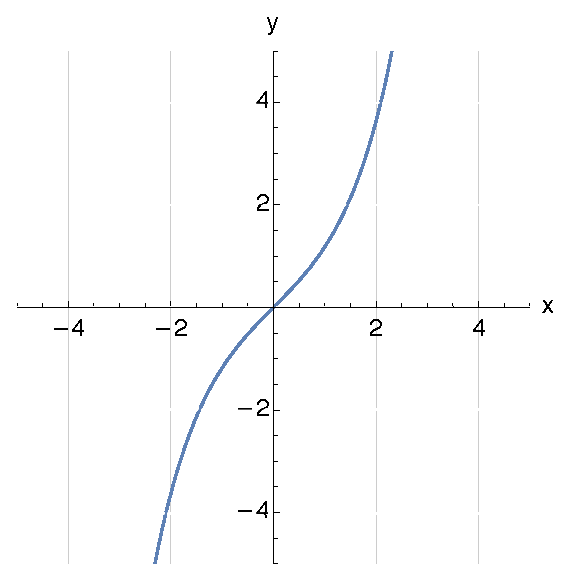
\includegraphics[height=4cm,width=4cm]{1.2.1.eps}
                          \caption{双曲正弦函数$y=\dfrac{e^x-e^{-x}}{2}$}
                      \end{minipage}%
                      \begin{minipage}[t]{0.5\linewidth}
                          \centering
                          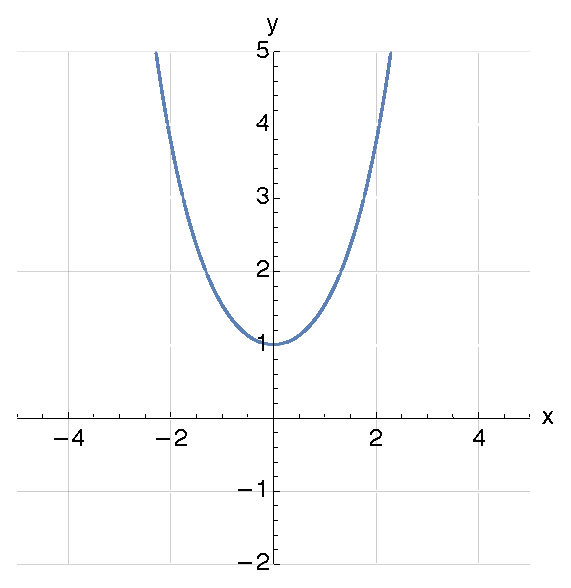
\includegraphics[height=4cm,width=4cm]{1.2.2.eps}
                          \caption{双曲余弦函数$y=\dfrac{e^x+e^{-x}}{2}$}
                      \end{minipage}
                  \end{figure}
            \item \textcolor{red}{下列有关反双曲正弦函数结论需要记住}
                  \begin{itemize}
                      \item $x\to0\text{时,}\ln\left(x+\sqrt{x^{2}+1}\right)\sim x.$
                      \item $\left[\ln\left(x+\sqrt{x^{2}+1}\right)\right]^{\prime}=\dfrac{1}{\sqrt{x^{2}+1}},\text{于是}\int\dfrac{1}{\sqrt{x^{2}+1}}dx=\ln\left(x+\sqrt{x^{2}+1}\right)+C.$
                      \item 由于$y=\ln\left(x+\sqrt{x^2+1}\right)$是奇函数,于是$\int_{-1}^1\left[\ln\left(x+\sqrt{x^2+1}\right)+x^2\right]\mathrm{d}x=\int_{-1}^1x^2\mathrm{d}x=\frac 23.$
                      \item 泰勒展开前两项为$x-\dfrac{1}{6}x^3$ \footnote{前两项和$\sin x$ 一样}
                  \end{itemize}
        \end{itemize}
    \end{note}
    \subsection{复合函数}
    设函数$y=f(u)$的定义域为$D_1$,函数$u=g(x)$在$D$上有定义,且$g(D) \subset D_1$,则由
    $$
        y=f[g(x)](x{\in}D)
    $$
    确定的函数,称为由函数$u=g(x)$和函数$y=f(u)$构成的\textbf{复合函数},它的定义域为D,u称为中间变量.内层函数的值域是外层函数的子集\footnote{需要注意的是,不是任何两个函数都可以进行复合,如果函数$A$的定义域与函数$B$的值域的交集为$\varnothing$,则两个函数不可进行复合}.
    \begin{problem}
    $\text{设}f(x)=\begin{cases}x^2,&x\geqslant0,\\x^4,&x<0,\end{cases}g(x)=\begin{cases}-\sqrt{x},&x>0,\\x^2,&x\leqslant0,\end{cases}\text{若}y=f(g(x)),$则
    \newline
    $(A)\frac{\mathrm{d}y}{\mathrm{d}x}\bigg|_{x=1}=1.\quad(\mathrm{B})\frac{\mathrm{d}y}{\mathrm{d}x}\bigg|_{x=1}\text{不存在}.\quad(\mathrm{C})\frac{\mathrm{d}y}{\mathrm{d}x}\bigg|_{x=0}=0.\quad(\mathrm{D})\frac{\mathrm{d}y}{\mathrm{d}x}\bigg|_{x=0}\text{不存在}.$
    \end{problem}
    \begin{solution}
        函数$y$为$f(x)$和$g(x)$复合函数,若求复合函数在$x=1$和$x=0$时的导数,那么可以将复合函数写为$f(x)=\begin{cases}g(x)^2,&x \geqslant 0\\g(x)^4,&x<0\end{cases}$,由此,作出$g(x)$函数图像,结合图像,可以将上述图像函数表达式更改为$f(g(x))=\begin{cases}x^2,&x\geqslant0\\x^4,&x<0\end{cases}$.则函数$f(g(x))$在$x=1$处的导数为0.
    \end{solution}
    \begin{note}
        看见复合函数,应把复合函数带入,把表达式求出来
    \end{note}
    \subsection{函数的四种特性及重要结论}
    \subsubsection{有界性}
    有界性分为三种情况,一种是有上界,一种是有下界,一种是有界。其中有界包含了有上界和有下界。
    \begin{defn}{有界性的定义}{}
        设$f(x)$的定义域为$D$,数集$I \subset D$.如果存在某个正数$M$,使对任一$x \in I$,有\textcolor{red}{$|f(x)| \leqslant M$},则称$f(z)$在$I$上\uwave{有界};如果这样的$M$不存在,则称$f(x)$在$I$上\uwave{无界}.
    \end{defn}
    \begin{itemize}\label{yjxpd1}
        \item \textbf{有界是指,同时有上界和下界}
        \item 从几何上看,如果在给定的区间,函数 $y=f(x)$的图形能够被直线 $y=-M$和 $y=M$"完全包起来",则为有界;从定义上说,找到某个正数 $M$,使得$|f(z)| \leqslant M$,则为有界.
        \item \textbf{在讨论有界还是无界的时候首先要指明区间},如果没指名区间,则无法讨论有界性.如函数$y=\dfrac{1}{x}$则$(2,+\infty)$上有界,但是在$(0,2)$上无界.
    \end{itemize}
   \subsubsection{\textcolor{red}{有界性的判断}}
        \begin{itemize}
            \item 利用定义
            \item $f(x)$在$[a,b]$上连续$\Rightarrow f(x)$在$[a,b]$上有界
            \item $f(x)$在$(a,b)$上连续,且$f(a^+)$和$f(b^-)$存在$\Leftrightarrow f(x)$在$(a,b)$上有界.
            \item \textbf{$f'(x)$在区间$I(\text{有限})$\footnote{长度有限}上有界$\Rightarrow f(x)$在$I$上有界}
                  \begin{proof}
                      \begin{itemize}
                          \item 使用拉格朗日中值定理进行证明:设区间$I(a,b)$由拉格朗日中值定理可得$f(b)-f(a)=f'(\xi)(b-a)$,固定点$a$,那么对区间$I(a,b)$上每一个点求拉格朗日中值定理,那么$f(x)=f(a)+f'(\xi)(x-a)$,其中$f(a)$为固定值,$(x-a)$为有界值,$f'(\xi)$在$I(a,b)$上有界,综上$f(x)$在区间上必有界。
                          \item 使用斜率进行证明:由几何意义可知,$f'(x)$为$f(x)$的斜率,那么如果$f'(x)$有界,那么斜率有界,那么说明$f(x)$的变化是有界的,那么更说明$f(x)$不可能无界。
                          \item 使用面积进行证明:$f'(x)$在有限区间上有界,则该区间上$f'(x)$与$x$轴所围成的面积是有界的,那么说明$f(x)$的变化是有界的,那么更说明$f(x)$不可能无界。
                      \end{itemize}
                  \end{proof}
        \end{itemize}
    \begin{problem}
    已知函数$f(x)=\dfrac{\int_0^x\ln(1+t^2)\operatorname{d}t}{x^a}\text{在}(0,+\infty)$上有界,则$a$的取值范围为
    \end{problem}
    \begin{solution}
        如果说$f(x)$在$(0,+\infty)$上有界,那么$f(x)$应该在区间两端点连续单侧极限存在.即$\lim_{x \to +\infty}f(x)$与$\lim_{x \to 0+}f(x)$极限存在。下面进行分情况讨论:
        \begin{align*}
            \lim_{x \to +\infty}f(x) & =\lim_{x \to +\infty}\dfrac{\int_0^x \ln(1+t^2)dt}{x^\alpha} \\
            & \xlongequal{\text{洛必达法则}}\lim_{x\to +\infty}\frac{\ln(1+x^2)}{\alpha x^{\alpha-1}}\\
            & =\lim_{x\to +\infty}\frac{\ln(1+x^2)}{\alpha x^{\alpha-1}}
        \end{align*}
        若要$x \to \infty$时函数有界,那么分母应趋近于无穷。则$\alpha -1>0$.\\
        \begin{align*}
            \lim_{x \to 0^+}f(x) & =\lim_{x \to 0^+}\frac{\int_0^x \ln(1+t^2)dt}{x^\alpha}   \\
            & \xlongequal{\text{洛必达法则}}\lim_{x \to 0^+}\frac{\ln(1+x^2)}{\alpha x ^\alpha-1}\\
            & \xlongequal{\text{等价无穷小}}\lim_{x\to 0^+}\frac{x^2}{\alpha x^{\alpha-1}}
        \end{align*}
        若要该极限成立。$\alpha -1\leqslant2$使得极限整体趋于0.综上所述,$\alpha$的取值范围应为$(1,3]$.
    \end{solution}
    \begin{problem}
    以下四个命题中正确的是:\\
    (A)若$f'(x)$在$(0,1)$内连续,则$f(x)$在$(0,1)$内有界\\
    (B)若$f(x)$在$(0,1)$内连续,则$f(x)$在$(0,1)$内有界\\
    (C)若$f'(x)$在$(0,1)$内有界,则$f(x)$在$(0,1)$内有界\\
    (D)若$f(x)$在$(0,1)$内有界,则$f'(x)$在$(0,1)$内有界
    \end{problem}
    \begin{solution}
        A,B选项.无论是导数还是原函数在区间上连续,都不可以推出原函数在区间上有界,比如函数$\frac{1}{x}$其在$(0,1)$区间上连续,但是其原函数$\ln x$在区间上无界.\\
        \textbf{一元函数中,优先看导数,由导数推函数\footnote{导数可以决定函数的变化,因此出现该类型的题目时,优先看有导数的选项}}。同时此处可以使用有界性判断\ref{yjxpd1}的定理三,可以得出导函数如果在有限区间$I$上有界,那么函数在区间$I$上有界。本题选C。
    \end{solution}
    \begin{problem}
    设函数$f(x)$连续,且$f'(0)>0$,则存在$\delta >0 $使得:\\
    (A)$f(x)$在$(0,\delta)$内单调增加\\
    (B)$f(x)$在$(0,\delta)$内单调减少\\
    (C)对任意的$x \in (0,\delta)$有$f(x)>f(0)$\\
    (D)对任意的$x\in (-\delta,0)$有$f(x)>f(0)$
    \end{problem}
    \begin{solution}
        \textbf{导数若存在,则导数要么连续,要么只可能有振荡间断点}。A,B选项\footnote{在本题中,答案给出了一个例子可以满足该题,即$\left.f\left(x\right)=\left\{\begin{matrix}x+2x^{2}\sin\frac{1}{x},&x\neq0,\\0,&x=0,\end{matrix}\right.\right.$,在考研中常用的一个例子是\textcolor{red}{$k \times \sin \dfrac{1}{x^b}\pm M \pm f(x)$}}:一点可导推不出区间可导,已知$f'(0)>0$那么假若函数$f(x)$在邻域内震荡,显然也满足$x=0$该点可导,但是在邻域内震荡,若$A$选项要正确.则需要增加条件$f(x)$在$x=0$处连续。$C,D$选项,由导数的定义得:$f'(0)=\lim_{x\to 0} \dfrac{f(x)-f(0)}{x}$。
    \end{solution}
    \subsubsection{单调性}
    \begin{defn}{单调性的定义}{}
        设$f(x)$的定义域为$D$,区间$I \subset D$.如果对于区间上任意两点$x_1,x_2$当$x_1 < x_2$时,恒有$f(x_1) < f(x_2)$,则称$f(x)$在区间$I$上\textbf{单调增加}.如果对于区间$I$上任意两点$x_1,x_2$当$x_1<x_2$,时,恒有$f(x_1)>f(x_2)$,则称$f(x)$在区间$I$上\textbf{单调减少}.
    \end{defn}
    判断单调性的方法
    \begin{enumerate}
        \item 利用导数进行判断,若$f(x)$在区间$I$上可导,则
        \begin{itemize}
            \item $f^{\prime}(x)>0(<0)\Rightarrow f(x)$ 单调增(单调减)
            \item $f^{\prime}(x)\geqslant0(\leqslant0)\Leftrightarrow f(x)$ 单调不减(单调不增)
        \end{itemize}
        \item 利用导数的定义,对任意$x_1,x_2\in D,x_1\neq x_2$,有
        \begin{itemize}
            \item $f\left(x\right)$是单调增函数(严格单调)$\Leftrightarrow\left(x_{1}-x_{2}\right)\left[f\left(x_{1}\right)-f\left(x_{2}\right)\right]>0$
            \item $f(x)$是单调减函数(严格单调)$\Leftrightarrow(x_{1}-x_{2})[f(x_{1})-f(x_{2})]<0$
            \item $f(x)$是单调不减函数$\Leftrightarrow(x_{1}-x_{2})[f(x_{1})-f(x_{2})]\geqslant0$
            \item $f\left(x\right)$是单调不增函数$\Leftrightarrow\left(x_{1}-x_{2}\right)\left[f\left(x_{1}\right)-f\left(x_{2}\right)\right]\leqslant0$
        \end{itemize}
    \end{enumerate}
    \subsubsection{奇偶性}
    \begin{defn}{奇偶性的定义}{}
        设$f(x)$的定义域$D$关于原点对称(即若$x \in D$,则$-x \in D$).如果对于任一$x \in D$,恒有$f(-x)=f(x)$,则称$f(x)$为\textbf{偶函数}.如果对于任一$x \in D$,恒有$f(-x)=-f(x)$,则称$f(x)$为\textbf{奇函数}.
    \end{defn}
    \begin{criterion}{奇偶性的性质}{}\label{jox2}
        \begin{enumerate}
            \item 奇偶函数运算后的奇偶性:
            \begin{itemize}
                \item 奇函数乘(除)偶函数=奇函数;
                \item 奇函数乘(除)奇函数=偶函数;
                \item 偶函数乘(除)偶函数=偶函数;
                \item 奇函数加(减)奇函数=奇函数;
                \item 偶函数加(减)偶函数=偶函数;
                \item 不恒为零的偶(奇)函数加减不恒为零的奇(偶)函数为非奇非偶函数;
                \item 偶(奇)函数乘以非奇非偶函数,一般不再是偶(奇)函数,为非奇非偶函数。
            \end{itemize}
            \item $f(\varphi(x))$(内偶则偶,内奇看外)\footnote{
                  奇[偶]$\Rightarrow$ 偶;偶[奇]$\Rightarrow$ 偶;奇[奇]$\Rightarrow$ 奇;偶[偶]$\Rightarrow$ 偶;非奇非偶[偶]$\Rightarrow$ 偶}
            \item 对任意的$x,y$都有$f(x+y)=f(x)+f(y)$,则$f(x)$是奇函数\footnote{证明如下:令$x=y=0$,则$f(0)=2*f(0)$,则$f(0)=0$,令$y=-x$,则$f(0)=f(x)+f(-x).$}.
            \item \textbf{求导后奇偶性互换}
            \item \textbf{连续的奇函数的一切原函数都是偶函数}\\\textbf{连续的偶函数的原函数中仅有一个原函数是奇函数\footnote{证明如下:设$f(x)$是连续函数,则其一个原函数可以表示为$F( x) = \int _a^xf( t) $d$t.$ 若$f(x)$是连续的奇函数,即有$f(x)=-f(-x)$,且$\int _{- a}^af( t) $d$t= 0$,则$F(-x)=\int_a^{-x} f(t) \mathrm{d} t \xlongequal{t=-u}-\int_{-a}^x f(-u) \mathrm{d} u=\int_{-a}^a f(u) \mathrm{d} u+\int_a^x f(u) \mathrm{d} u=0+F(x)=F(x)$.若$f(x)$是连续的偶函数,即有$f(-x)=f(x)$,且$\int _{- a}^af( t) $d$t= 2\int _0^af( t) $d$t$,则$F(-x)=\int_a^{-x} f(t) \mathrm{d} t \xlongequal{t=-u}-\int_{-a}^x f(-u) \mathrm{d} u=-\int_{-a}^a f(u) \mathrm{d} u-\int_a^x f(u) \mathrm{d} u=-2 \int_0^a f(u) \mathrm{d} u-F(x)$则当$\int _0 ^a f(u)du \equiv 0$时,F(x)为奇函数.}}\label{jox1}
            \item \textbf{设$f(x)$连续,若$f(x)$是奇函数,则$\int_{a}^{x}f\left(t\right)\mathrm{d}t$是偶函数;\\若$f(x)$是偶函数,则$\int_{0}^{x}f\left(t\right)\mathrm{d}t$是奇函数}\footnote{证明如下:设$F(x)=\int_a ^x f(t)dt$由变上限积分求导公式可得:$(\int _a ^x f(t)dt)'=f(x)$,已知$f(x)$为奇/偶函数,由奇偶性的性质 \ref{jox2} 中第\ref{jox1}条可得}
            \item \textbf{对于任意函数$f(x)$,令$u(x)=\dfrac{1}{2}[f(x)+f(-x)]$,$v(x)=\dfrac{1}{2}[f(x)-f(-x)]$,其中,$u(x)$是偶函数,$v(x)$是奇函数.因为$f(x)=\dfrac{1}{2}[f(x)+f(-x)]+\dfrac{1}{2}[f(x)-f(-x)]=u(x)+v(x)$}
            \item 奇函数$y=f(x)$的图形关于坐标原点对称,当$f(x)$在$x=0$处有定义时,必有$f(0)=0$.
            \item 偶函数$y=f(x)$的图形关于$y$轴对称,且当$f(0)$存在时,必有$f'(0)=0$.
            \item 设$f(x)$是定义在$[-l,l]$上的任意函数,则
                  $$
                      F_1(x)=f(x)-f(-x)\text{必为奇函数};F_2(x)=f(x)+f(-x)\text{必为偶函数}\footnote{证明如下:已知$f(x)$是任意函数,$-1$带入可得,$F_1(-x)=f(-x)-f(x)=-F_1(x)$,同理可证$F_2$成立.}
                  $$
        \end{enumerate}
    \end{criterion}
    \begin{problem}
    设$f(x)$连续且为奇函数,则下列函数中必为偶函数的为\\
    (A) $\int_0 ^x du \int _a ^u t f(t) dt$ \qquad \qquad (B)$\int_a ^x du \int _0 ^u f(t)dt$\\
    (C) $\int _a ^x du \int _0 ^u tf(t)dt$  \qquad \qquad (D) $\int_0 ^x du \int _a ^u f(t) dt$
    \end{problem}
    \begin{solution}
       $A$选项 已知函数$f(x)$连续为奇函数,那么$tf(t)$为偶函数,若其想为奇函数,其积分形式应为$\int _0 ^u tf(t) dt$.\\ $B$选项为奇函数,$\int _0 ^x f(t) dt$为偶函数,再次积分,无法满足过原点,因此无奇偶性.
       \\$C$选项,同理,$tf(t)$为偶函数,积分后为奇函数,再次积分后为偶函数,正确
       \\$D$选项,第一次积分后为非奇非偶函数
    \end{solution}
    \subsubsection{周期性}
    \begin{defn}{周期函数的定义}{}
        设$f(x)$的定义域为$D$,如果存在一个正数$T$,使得对于任一$x \in D$,有$x \pm T \in D$,且$f(x+T)=f(x)$,则称$f(x)$为周期函数,$T$称为$f(x)$的周期.从几何图形上看,在周期函数的定义域内,相邻两个长度为$T$的区间上,函数的图形完全一样.
    \end{defn}
    需要注意的是函数的周期性只与$x$的参数有关,比如若函数$f(x)$以$T$为周期,则$f(ax+b)$以$\frac{T}{|a|}$为周期.\textbf{可以观察到其周期只与$x$的系数有关}
    \subsubsection{重要结论}
    \begin{itemize}
        \item 若$f(x)$是可导的周期为$T$的周期函数,则$f'(x)$也是以$T$为周期的周期函数.\label{zyjl1}
        \item 设$f(x)$\textbf{连续且以$T$为周期,则$F(x)=\int_0 ^x f(t)dt$ 是以$T$为周期的周期函数$\Leftrightarrow\int_{0}^{\tau}f(x)\mathrm{d}x=0.$}\footnote{证明如下:$F(x+T)=\int_{a}^{x+T}f(t)\mathrm{d}t=\int_{a}^{x}f(t)\mathrm{d}t+\int_{x}^{x+T}f(t)\mathrm{d}t$,因为$f(x)$ 以$T$为周期,于是$\int _x^{x+ T}f( t) $d$t= \int _0^Tf( t) $d$t$, 即$F( x+ T) - F( x) = \int _0^Tf( t) $d$t$,所以当且仅当$\int _0^Tf( t) $d$t= 0, $即$\int _0^Tf( x) $d$x= 0$ 时,$F(x)$ 以$T$为周期.}
        \item \textbf{周期函数的原函数是周期函数的充要条件是其在一个周期上的积分为0.}\label{zyjl2}
    \end{itemize}
    \subsubsection{周期性的判断}
    \begin{enumerate}
        \item 利用周期性的定义
        \item 根据定义\ref{zyjl1}第一条可导的周期函数其导函数为周期函数
        \item 根据定义\ref{zyjl2}第三条周期函数的原函数不一定是周期函数\footnote{如函数$1+\cos x$}
    \end{enumerate}
    \subsection{三种特殊函数}
    \subsubsection{符号函数}
    $$
        y=\text{sgn} \ x=\begin{cases}-1,&x<0,\\0,&x=0,\\1,&x>0\end{cases}
    $$
    \begin{center}
        \tikzset{every picture/.style={line width=0.75pt}} %set default line width to 0.75pt        
        \begin{tikzpicture}[x=0.75pt,y=0.75pt,yscale=-1,xscale=1]
            \draw  (144,128.43) -- (426.14,128.43)(283.14,38.43) -- (283.14,201) (419.14,123.43) -- (426.14,128.43) -- (419.14,133.43) (278.14,45.43) -- (283.14,38.43) -- (288.14,45.43) (303.14,123.43) -- (303.14,133.43)(323.14,123.43) -- (323.14,133.43)(343.14,123.43) -- (343.14,133.43)(363.14,123.43) -- (363.14,133.43)(383.14,123.43) -- (383.14,133.43)(403.14,123.43) -- (403.14,133.43)(263.14,123.43) -- (263.14,133.43)(243.14,123.43) -- (243.14,133.43)(223.14,123.43) -- (223.14,133.43)(203.14,123.43) -- (203.14,133.43)(183.14,123.43) -- (183.14,133.43)(163.14,123.43) -- (163.14,133.43)(278.14,108.43) -- (288.14,108.43)(278.14,88.43) -- (288.14,88.43)(278.14,68.43) -- (288.14,68.43)(278.14,148.43) -- (288.14,148.43)(278.14,168.43) -- (288.14,168.43)(278.14,188.43) -- (288.14,188.43) ;
            \draw   ;
            \draw    (285.14,88.43) -- (420.29,88.43) ;
            \draw    (146.14,168.43) -- (281.29,168.43) ;
            \draw  [fill={rgb, 255:red, 0; green, 0; blue, 0 }  ,fill opacity=1 ] (280.65,130.46) .. controls (279.52,129.09) and (279.73,127.06) .. (281.11,125.93) .. controls (282.48,124.81) and (284.51,125.02) .. (285.64,126.39) .. controls (286.76,127.77) and (286.56,129.8) .. (285.18,130.92) .. controls (283.8,132.05) and (281.77,131.84) .. (280.65,130.46) -- cycle ;
            \draw  [fill={rgb, 255:red, 255; green, 255; blue, 255 }  ,fill opacity=1 ] (280.61,87.97) .. controls (279.49,86.59) and (279.69,84.57) .. (281.07,83.44) .. controls (282.45,82.32) and (284.48,82.52) .. (285.6,83.9) .. controls (286.73,85.28) and (286.52,87.3) .. (285.14,88.43) .. controls (283.77,89.55) and (281.74,89.35) .. (280.61,87.97) -- cycle ;
            \draw  [fill={rgb, 255:red, 255; green, 255; blue, 255 }  ,fill opacity=1 ] (281.29,168.43) .. controls (280.16,167.05) and (280.37,165.02) .. (281.74,163.9) .. controls (283.12,162.77) and (285.15,162.98) .. (286.27,164.36) .. controls (287.4,165.73) and (287.19,167.76) .. (285.82,168.89) .. controls (284.44,170.01) and (282.41,169.81) .. (281.29,168.43) -- cycle ;
            \draw (280,15) node [anchor=north west][inner sep=0.75pt]   [align=left] {$\displaystyle y$};
            \draw (433,117) node [anchor=north west][inner sep=0.75pt]   [align=left] {$\displaystyle x$};
        \end{tikzpicture}
    \end{center}
    \subsubsection{取整函数}
    $$
        y=[x]
    $$
    数值上向下取整,数轴上向左取整\footnote{\textbf{坐标轴上向左移,在现实生活中就是年龄}},即$x-1<[x] \leq x$
    \begin{center}
        \tikzset{every picture/.style={line width=0.75pt}} %set default line width to 0.75pt        
        \begin{tikzpicture}[x=0.75pt,y=0.75pt,yscale=-1,xscale=1]
            \draw  (124,139.63) -- (359,139.63)(239.82,39.5) -- (239.82,236.5) (352,134.63) -- (359,139.63) -- (352,144.63) (234.82,46.5) -- (239.82,39.5) -- (244.82,46.5) (259.82,134.63) -- (259.82,144.63)(279.82,134.63) -- (279.82,144.63)(299.82,134.63) -- (299.82,144.63)(319.82,134.63) -- (319.82,144.63)(339.82,134.63) -- (339.82,144.63)(219.82,134.63) -- (219.82,144.63)(199.82,134.63) -- (199.82,144.63)(179.82,134.63) -- (179.82,144.63)(159.82,134.63) -- (159.82,144.63)(139.82,134.63) -- (139.82,144.63)(234.82,119.63) -- (244.82,119.63)(234.82,99.63) -- (244.82,99.63)(234.82,79.63) -- (244.82,79.63)(234.82,59.63) -- (244.82,59.63)(234.82,159.63) -- (244.82,159.63)(234.82,179.63) -- (244.82,179.63)(234.82,199.63) -- (244.82,199.63)(234.82,219.63) -- (244.82,219.63) ;
            \draw   ;
            \draw [color={rgb, 255:red, 208; green, 2; blue, 27 }  ,draw opacity=1 ]   (260.13,120.19) -- (278.63,120.19) ;
            \draw  [color={rgb, 255:red, 208; green, 2; blue, 27 }  ,draw opacity=1 ] (278.63,120.19) .. controls (278.63,119.26) and (279.38,118.5) .. (280.31,118.5) .. controls (281.24,118.5) and (282,119.26) .. (282,120.19) .. controls (282,121.12) and (281.24,121.88) .. (280.31,121.88) .. controls (279.38,121.88) and (278.63,121.12) .. (278.63,120.19) -- cycle ;
            \draw [color={rgb, 255:red, 208; green, 2; blue, 27 }  ,draw opacity=1 ]   (239.38,139.44) -- (257.88,139.44) ;
            \draw  [color={rgb, 255:red, 208; green, 2; blue, 27 }  ,draw opacity=1 ] (257.88,139.44) .. controls (257.88,138.51) and (258.63,137.75) .. (259.56,137.75) .. controls (260.49,137.75) and (261.25,138.51) .. (261.25,139.44) .. controls (261.25,140.37) and (260.49,141.13) .. (259.56,141.13) .. controls (258.63,141.13) and (257.88,140.37) .. (257.88,139.44) -- cycle ;
            \draw [color={rgb, 255:red, 208; green, 2; blue, 27 }  ,draw opacity=1 ]   (280.13,100.19) -- (298.63,100.19) ;
            \draw  [color={rgb, 255:red, 208; green, 2; blue, 27 }  ,draw opacity=1 ] (298.63,100.19) .. controls (298.63,99.26) and (299.38,98.5) .. (300.31,98.5) .. controls (301.24,98.5) and (302,99.26) .. (302,100.19) .. controls (302,101.12) and (301.24,101.88) .. (300.31,101.88) .. controls (299.38,101.88) and (298.63,101.12) .. (298.63,100.19) -- cycle ;
            \draw [color={rgb, 255:red, 208; green, 2; blue, 27 }  ,draw opacity=1 ]   (299.63,80.44) -- (318.13,80.44) ;
            \draw  [color={rgb, 255:red, 208; green, 2; blue, 27 }  ,draw opacity=1 ] (318.13,80.44) .. controls (318.13,79.51) and (318.88,78.75) .. (319.81,78.75) .. controls (320.74,78.75) and (321.5,79.51) .. (321.5,80.44) .. controls (321.5,81.37) and (320.74,82.13) .. (319.81,82.13) .. controls (318.88,82.13) and (318.13,81.37) .. (318.13,80.44) -- cycle ;
            \draw [color={rgb, 255:red, 208; green, 2; blue, 27 }  ,draw opacity=1 ]   (320.13,60.19) -- (338.63,60.19) ;
            \draw  [color={rgb, 255:red, 208; green, 2; blue, 27 }  ,draw opacity=1 ] (338.63,60.19) .. controls (338.63,59.26) and (339.38,58.5) .. (340.31,58.5) .. controls (341.24,58.5) and (342,59.26) .. (342,60.19) .. controls (342,61.12) and (341.24,61.88) .. (340.31,61.88) .. controls (339.38,61.88) and (338.63,61.12) .. (338.63,60.19) -- cycle ;
            \draw [color={rgb, 255:red, 208; green, 2; blue, 27 }  ,draw opacity=1 ]   (219.63,159.63) -- (238.13,159.63) ;
            \draw  [color={rgb, 255:red, 208; green, 2; blue, 27 }  ,draw opacity=1 ] (238.13,159.63) .. controls (238.13,158.69) and (238.88,157.94) .. (239.81,157.94) .. controls (240.74,157.94) and (241.5,158.69) .. (241.5,159.63) .. controls (241.5,160.56) and (240.74,161.31) .. (239.81,161.31) .. controls (238.88,161.31) and (238.13,160.56) .. (238.13,159.63) -- cycle ;
            \draw [color={rgb, 255:red, 208; green, 2; blue, 27 }  ,draw opacity=1 ]   (199.88,180.13) -- (218.38,180.13) ;
            \draw  [color={rgb, 255:red, 208; green, 2; blue, 27 }  ,draw opacity=1 ] (218.38,180.13) .. controls (218.38,179.19) and (219.13,178.44) .. (220.06,178.44) .. controls (220.99,178.44) and (221.75,179.19) .. (221.75,180.13) .. controls (221.75,181.06) and (220.99,181.81) .. (220.06,181.81) .. controls (219.13,181.81) and (218.38,181.06) .. (218.38,180.13) -- cycle ;
            \draw [color={rgb, 255:red, 208; green, 2; blue, 27 }  ,draw opacity=1 ]   (179.75,199.75) -- (198.25,199.75) ;
            \draw  [color={rgb, 255:red, 208; green, 2; blue, 27 }  ,draw opacity=1 ] (198.25,199.75) .. controls (198.25,198.82) and (199.01,198.06) .. (199.94,198.06) .. controls (200.87,198.06) and (201.63,198.82) .. (201.63,199.75) .. controls (201.63,200.68) and (200.87,201.44) .. (199.94,201.44) .. controls (199.01,201.44) and (198.25,200.68) .. (198.25,199.75) -- cycle ;
            \draw [color={rgb, 255:red, 208; green, 2; blue, 27 }  ,draw opacity=1 ]   (159.75,220.25) -- (178.25,220.25) ;
            \draw  [color={rgb, 255:red, 208; green, 2; blue, 27 }  ,draw opacity=1 ] (178.25,220.25) .. controls (178.25,219.32) and (179.01,218.56) .. (179.94,218.56) .. controls (180.87,218.56) and (181.63,219.32) .. (181.63,220.25) .. controls (181.63,221.18) and (180.87,221.94) .. (179.94,221.94) .. controls (179.01,221.94) and (178.25,221.18) .. (178.25,220.25) -- cycle ;
            \draw (235,11) node [anchor=north west][inner sep=0.75pt]   [align=left] {y};
            % Text Node
            \draw (363,130) node [anchor=north west][inner sep=0.75pt]   [align=left] {x};
        \end{tikzpicture}
    \end{center}

    \subsubsection{狄利克雷函数}\footnote{本函数图像无法绘制}
    $$
        D\left(x\right)=\left\{\begin{matrix}{1,}&x\in\mathbf{Q},\\{0,}&x\in\mathbf{Q}^{c}.\end{matrix}\right.
    $$

    \section{函数图像}
    \subsection{常数函数}
    $y=A$,$A$为常数,其图形为平行于$x$轴的水平直线
    \begin{figure}[H]
        \centering 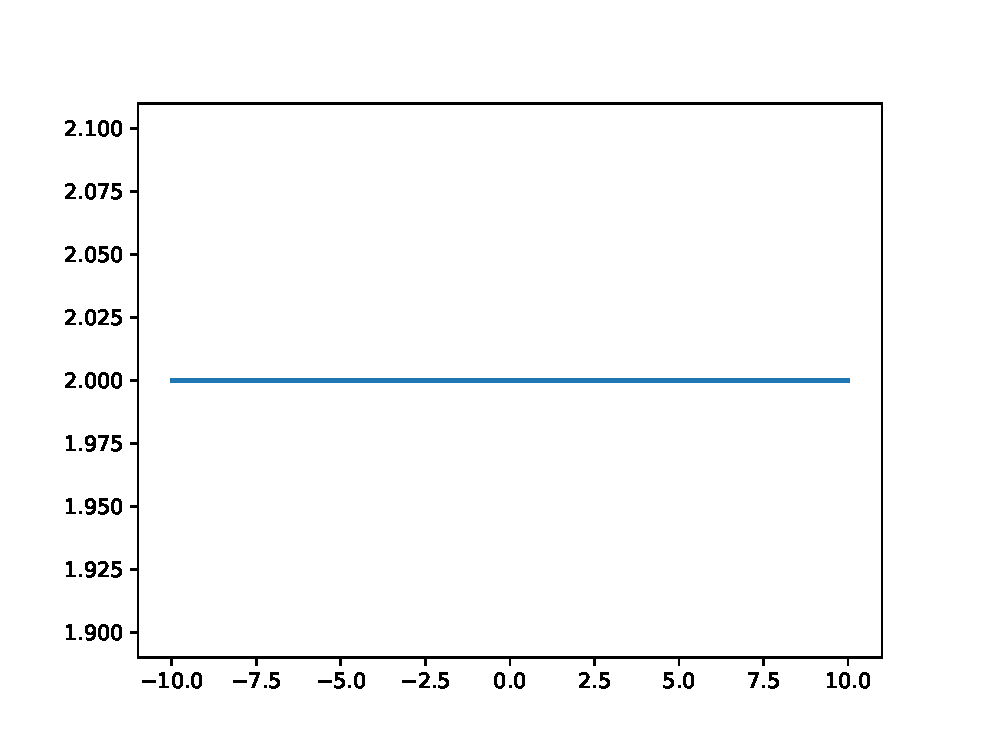
\includegraphics[width=
            0.55 \linewidth]{1.3.1.eps} \caption{常数函数图像}
    \end{figure}
    \subsection{幂函数}
    $$
        y=x^{\mu}(\mu \text{是实数})
    $$
    \begin{figure}[H]
        \centering
        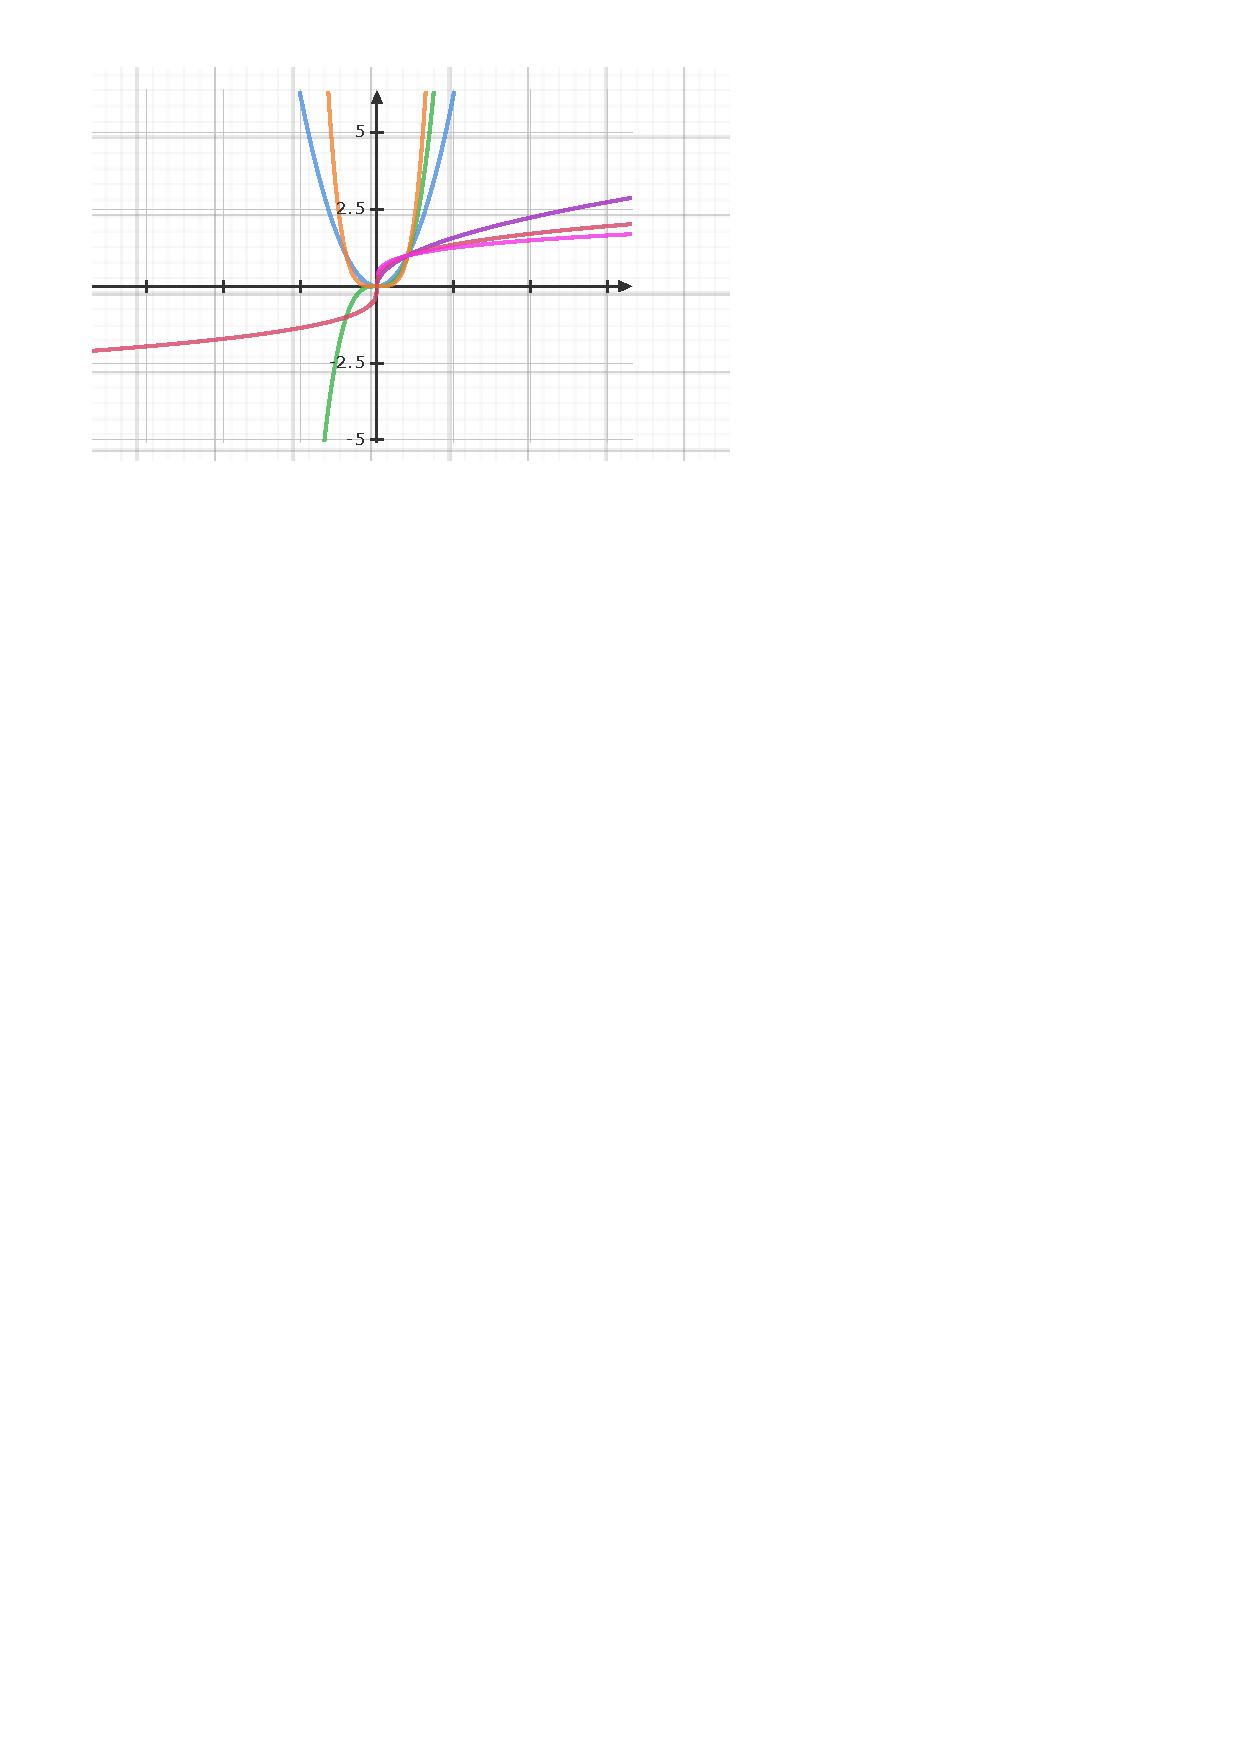
\includegraphics[width=0.8\textwidth]{1.3.2.1.pdf}
        \caption{幂函数图像}
    \end{figure}
    \begin{criterion}{幂函数常用技巧}{}
        \begin{itemize}
            \item 当$\mu>0$且$0<x<1$时,函数随着$\mu$的增大而变小(越大越低)
            \item 当$\mu >0$且$x>1$时,函数随着$\mu$的增大而变大(越大越高)
            \item 当$\mu <0$且$0<x<1$时,函数随着$\mu$的增大而变小(越大越低)
            \item 当$\mu <0$且$x>1$时,函数随着$\mu$的增大而变大(越大越高)
            \item 当$x>0$时,由$y=x$与$y=\sqrt{x}$,$y=\sqrt[3]{x}$,$y=\ln x$具有相同的单调性,因此可以利用这一特性来研究最值
            \item 见到$\sqrt{u}$,$\sqrt[3]{u}$时,可用$u$来研究最值
            \item 见到$\mid u\mid$时,由$\mid u\mid=\sqrt{u^2}$,可用 $u^2$ 来研究最值
            \item 见到$u_1,u_2,u_3$,$\ln (u_1+u_2+u_3)=\ln u_{1}+\ln u_{2}+\ln u_{3}$来研究最值
            \item 见到$\dfrac{1}{u}$时,可用$u$来研究最值(结论相反),即$\dfrac{1}{u}$与$u$的最大值点、最小值点相反
        \end{itemize}
    \end{criterion}
    \subsection{指数函数}
    $$
        y=a^x (a>0,a \neq 1)
    $$
    \begin{figure}[H]
        \centering 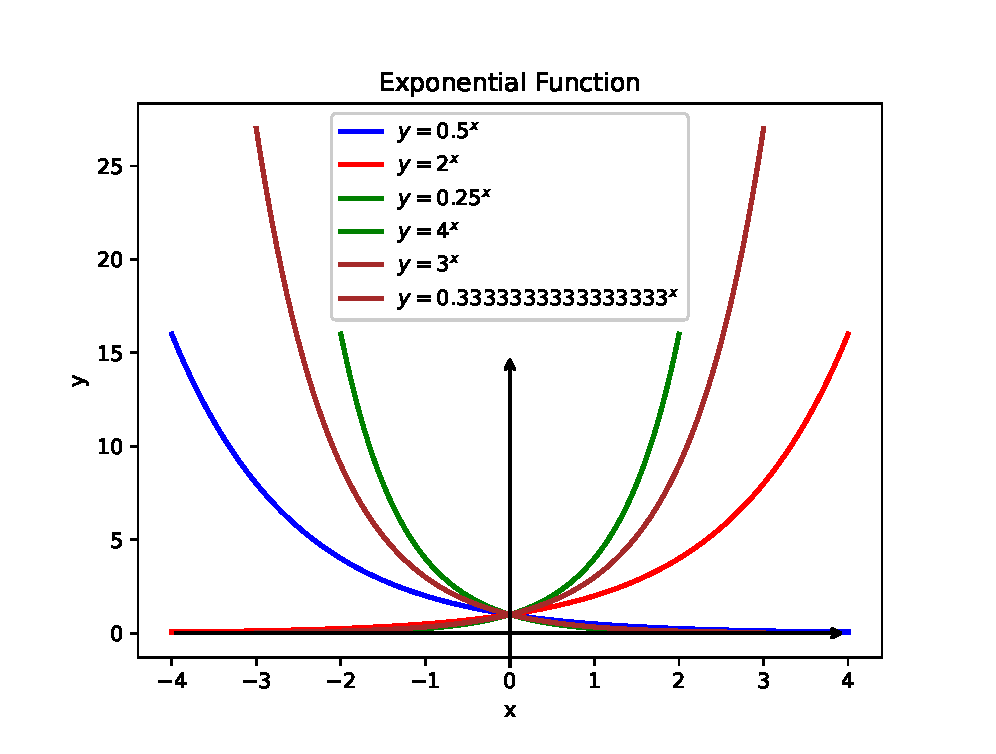
\includegraphics[width=
            0.5 \linewidth]{1.3.2.eps} \caption{指数函数图像}
    \end{figure}
    \begin{criterion}{指数函数相关性质}{}
        \begin{itemize}
            \item 定义域:$(-\infty,+\infty)$.值域:$(0,+\infty)$.
            \item 单调性:常用的指数函数$y=\mathrm{e}^x$
            \item 极限:$\lim_{x\to-\infty}\mathrm{e}^x=0,\lim_{x\to+\infty}\mathrm{e}^x=+\infty$(由于极限的唯一性,因此在趋于不同的无穷时,极限值的不同).
            \item 特殊函数值:$a^0=1$,$\mathrm{e}^0=1$
            \item 指数运算法则:
                  $$
                      a^{\alpha}\times a^{\beta}=a^{\alpha+\beta},\frac{a^{\alpha}}{a^{\beta}}=a^{\alpha-\beta}\footnote{$eg:e^{\tan x}-e^{\sin x}=e^{\sin x}\left(e^{\tan x-\sin x}-1\right)$},(a^{\alpha})^{\beta}=a^{\alpha\beta},(ab)^{\alpha}=a^{\alpha}b^{\alpha},\left(\dfrac{a}{b}\right)^{\alpha}=\dfrac{a^{\alpha}}{b^{\alpha}},
                  $$
        \end{itemize}
    \end{criterion}
    \subsection{对数函数}
    $$
        y=\log_a x (a>0,a \neq 1)
    $$
    \begin{figure}[H]
        \centering 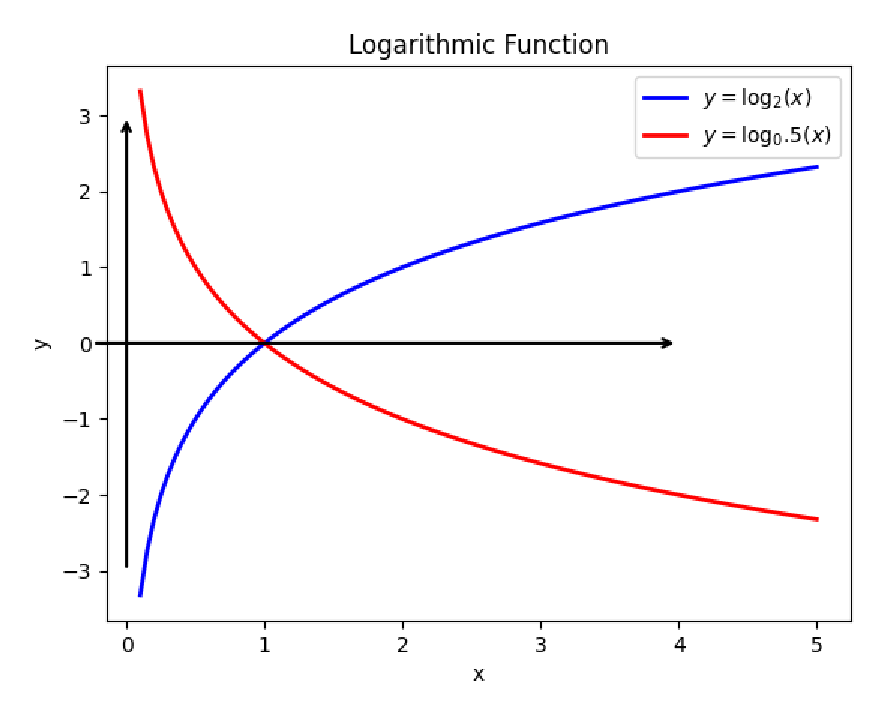
\includegraphics[width=
            0.5 \linewidth]{1.3.3.eps} \caption{对数函数图像}
    \end{figure}
    \begin{criterion}{对数函数相关性质}{}
        \begin{itemize}
            \item 定义域:$(0,+\infty)$.值域:$(-\infty,+\infty)$.
            \item 单调性:当 $a>1$时,$y=log_a x$单调增加;当$0<a<1$时,$y=\log_a x$单调减少;
            \item 常用对数函数: $y=\ln x$
            \item 特殊函数值:$\log_a 1=0$,$\log_a=1$,$\ln 1=0$,$\ln e=1$
            \item 极限$\operatorname*{lim ln}_{x\to0^{+}}x=-\infty$,$\operatorname*{lim ln}_{x\to+\infty}x=+\infty$.
            \item 对数运算法则
                  \begin{itemize}
                      \item $\log_{a}\left(MN\right)=\log_{a}M+\log_{a}N\left(\text{ 积的对数}=\text{对数的和 }\right).$
                      \item $\log_{a}\dfrac{M}{N}=\log_{a}M-\log_{a}N\left(\text{商的对数}=\text{对数的差 }\right).$
                      \item $\log_aM^n=n\log_aM,\quad\log_a\sqrt[n]{M}=\frac1n\log_aM\text{(幂的对数}=\text{对数的倍数 }).$
                  \end{itemize}
            \item \textcolor{red}{常用公式:$x=\mathrm{e}^{\ln x}\left(x>0\right),u^{\upsilon}=\mathrm{e}^{\ln u^v}=\mathrm{e}^{\upsilon\ln u}\left(u>0\right)$}
            \item 当$x>0$时,常用于中值定理:
                  $$
                      \ln\sqrt{x}=\frac{1}{2}\ln x;\ln\frac{1}{x}=-\ln x;\ln\biggl(1+\frac{1}{x}\biggr)=\ln\frac{x+1}{x}=\ln(x+1)-\ln x.
                  $$
        \end{itemize}
    \end{criterion}
    \subsection{三角函数}

    \subsubsection{正弦和余弦函数}
    $$
        \boxed{y=\sin x}
        \qquad \qquad \qquad \qquad \qquad \qquad \qquad \qquad
        \boxed{y=\cos x}
    $$
    \begin{figure}[H] \centering
        \subfigure[正弦函数图像] {
            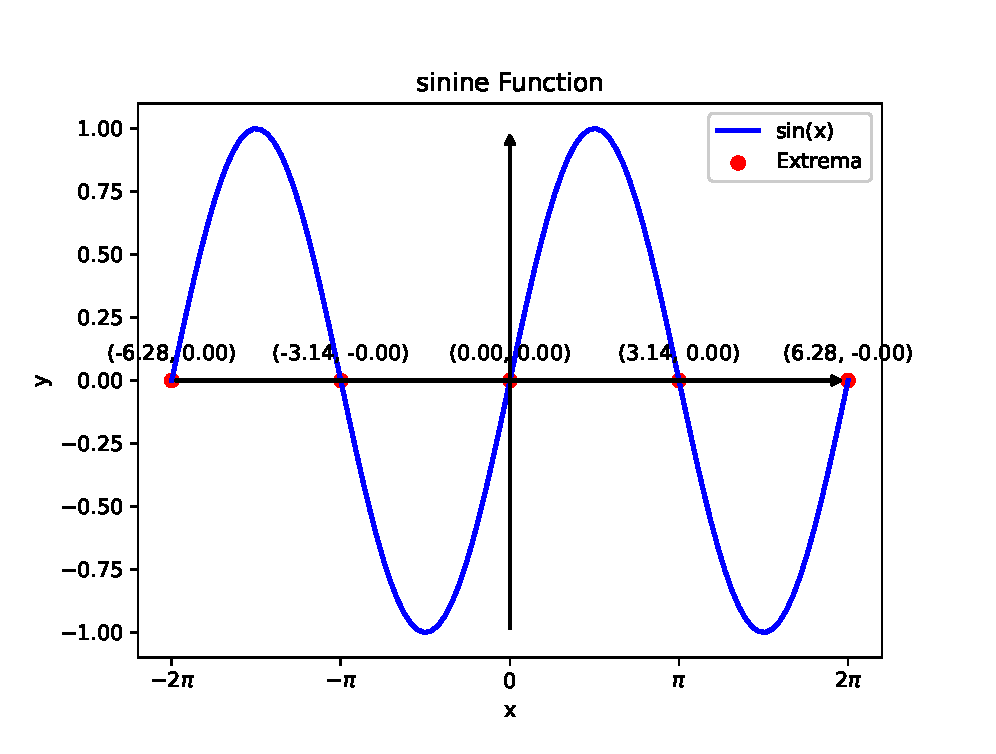
\includegraphics[width=0.45\columnwidth]{1.3.5.eps}
        }
        \subfigure[余弦函数图像] {
            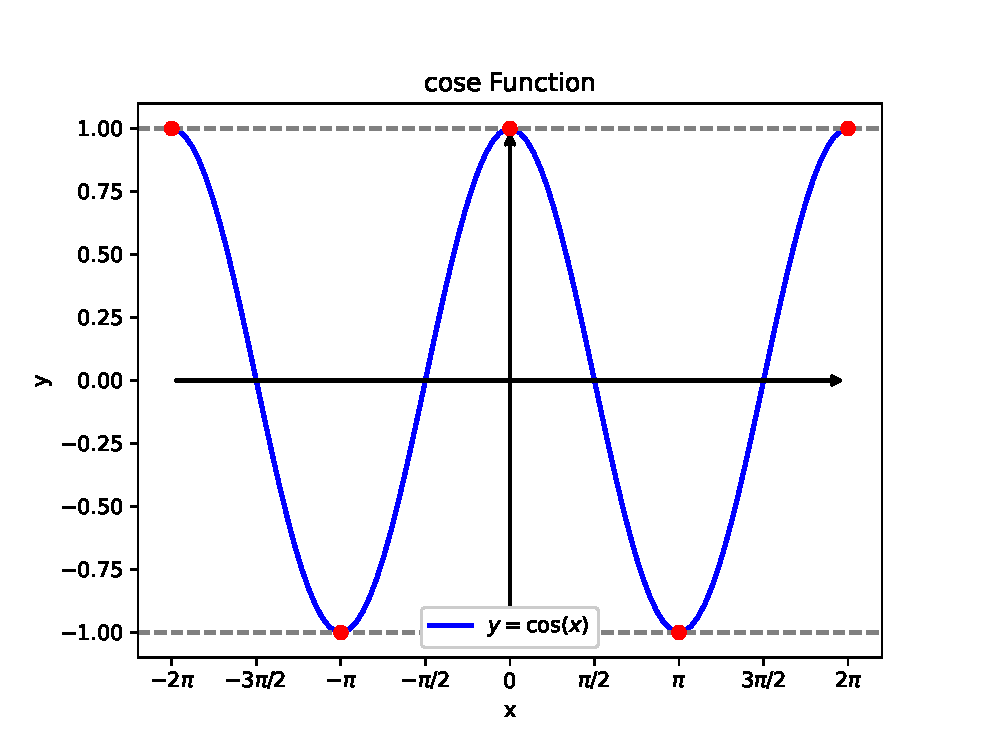
\includegraphics[width=0.45\columnwidth]{1.3.4.eps}
        }
        \caption{正余弦函数图像}
    \end{figure}
    \begin{criterion}{正余弦函数相关性质}{}
        \begin{itemize}
            \item 定义域:$(-\infty,+\infty)$,值域:$[-1,1]$
            \item 奇偶性:$y=\sin x$是奇函数,$y=\cos x$是偶函数,$x\in (-\infty,+\infty)$
            \item 周期性:$y=\sin x$和$y=\cos x$均以$2\pi$为最小正周期.$x\in (-\infty,+\infty)$
            \item 有界性:$\left|\sin x\right|\leqslant1,\left|\cos x\right|\leqslant1$
            \item $\sin^{2}\alpha+\cos^{2}\alpha=1$
        \end{itemize}
    \end{criterion}
    \subsubsection{正切和余切函数}
    $$
        \boxed{y=\tan x=\frac{\sin x}{\cos x}}
        \qquad \qquad \qquad \qquad \qquad \qquad \qquad \qquad
        \boxed{y=\cot x=\frac{\cos x}{\sin x}=\frac{1}{\tan x}}
    $$
    \begin{figure}[H] \centering
        \subfigure[正切函数图像] {
            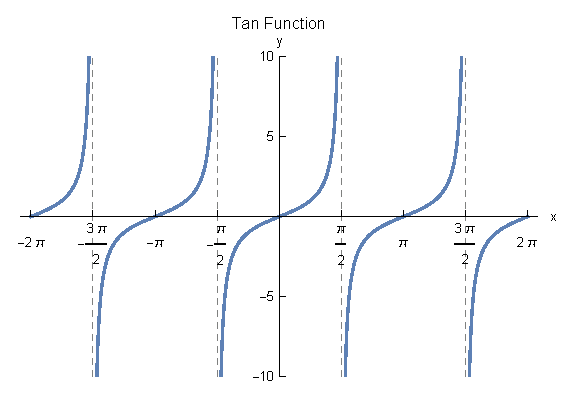
\includegraphics[width=0.45\columnwidth]{1.3.6.eps}
        }
        \subfigure[余切函数图像] {
            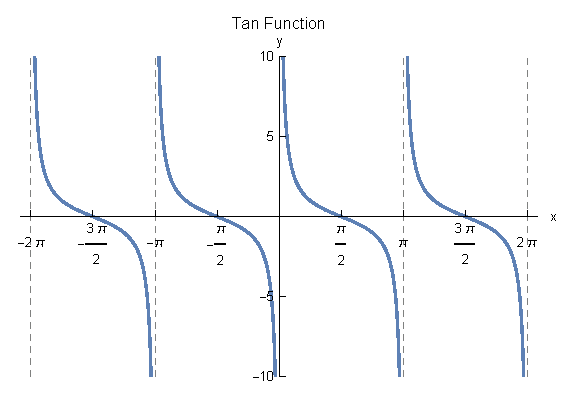
\includegraphics[width=0.45\columnwidth]{1.3.7.eps}
        }
        \caption{正余切函数图像}
    \end{figure}
    \begin{criterion}{正余切函数相关性质}{}
        \begin{itemize}
            \item $y=\tan x$的定义域为$\left\{x\left|x\neq k\pi+\frac{\pi}{2}\left(k\in\mathbf{Z}\right)\right\}\right.$;\\$y=\cot x$的定义域为$\left\{x\left|x\neq k\pi+\left(k\in\mathbf{Z}\right)\right\}\right.$;\\
                      值域均为$(-\infty,+\infty)$
            \item 奇偶性:均为奇函数
            \item 周期性:均以$\pi$为最小正周期
        \end{itemize}
    \end{criterion}

    \subsubsection{正割和余割函数}
    $$
        \boxed{\sec x=\frac{1}{\cos x}}
        \qquad  \qquad \qquad \qquad \qquad \qquad
        \boxed{\csc x=\frac{1}{\sin x}}
    $$
    \begin{figure}[H] \centering
        \subfigure[正割函数图像] {
            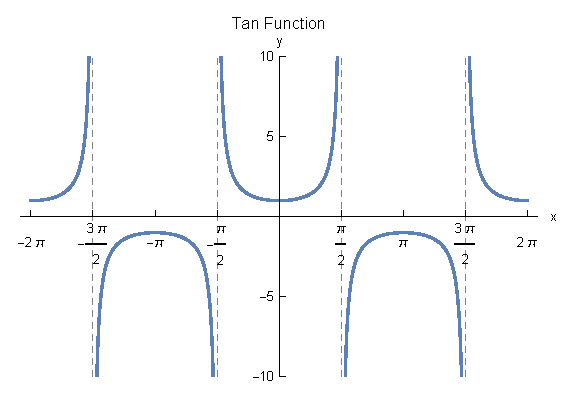
\includegraphics[width=0.4\columnwidth]{1.3.8.eps}
        }
        \subfigure[余割函数图像] {
            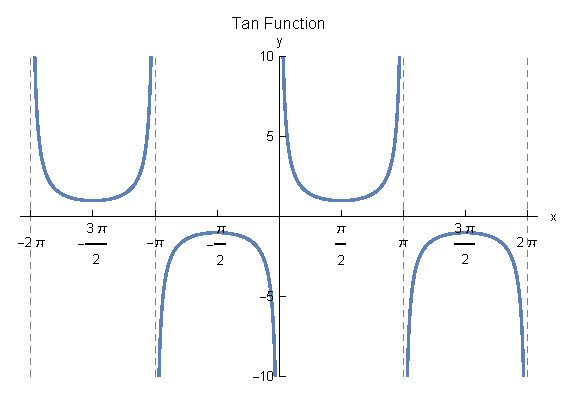
\includegraphics[width=0.4\columnwidth]{1.3.9.eps}
        }
        \caption{正余割函数图像}
    \end{figure}
    \begin{criterion}{正余割函数相关性质}{}
        \begin{itemize}
            \item 定义域:$y=\sec x$的定义域是$\left\{x\left|x\neq k\pi+\dfrac{\pi}{2}\left(k\in\mathbf{Z}\right)\right\}\right.$;$y=\csc x$ 的定义域为$\{x|x\neq k\pi,(k \in \mathbf{Z})\}$值域均为:$(-\infty,-1]\cup[1,+\infty)$
            \item 奇偶性:$y=\sec x$为偶函数,$y=\csc x$为奇函数
            \item 周期性:最小正周期均为$ 2\pi$
            \item $1+\tan^{2}\alpha=\sec^{2}\alpha;1+\cot^{2}\alpha=\csc^{2}\alpha $
        \end{itemize}
    \end{criterion}
    \subsubsection{反三角函数}
    \subsubsection{反正弦和反余弦函数}
    $$
        \boxed{y=\arcsin x}
        \qquad \qquad \qquad \qquad \qquad \qquad
        \boxed{y=\arccos x}
    $$
    \begin{figure}[H] \centering
        \subfigure[反正弦函数图像] {
            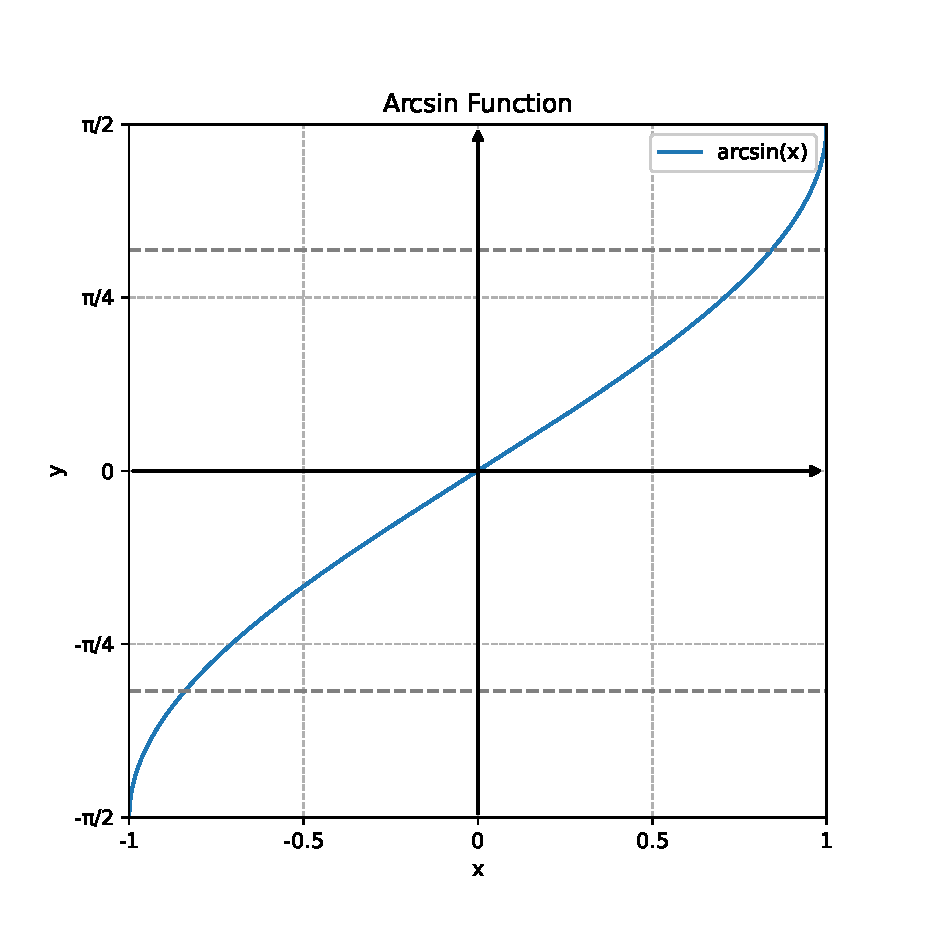
\includegraphics[width=0.4\columnwidth]{1.3.10.eps}
        }
        \subfigure[反余弦函数图像] {
            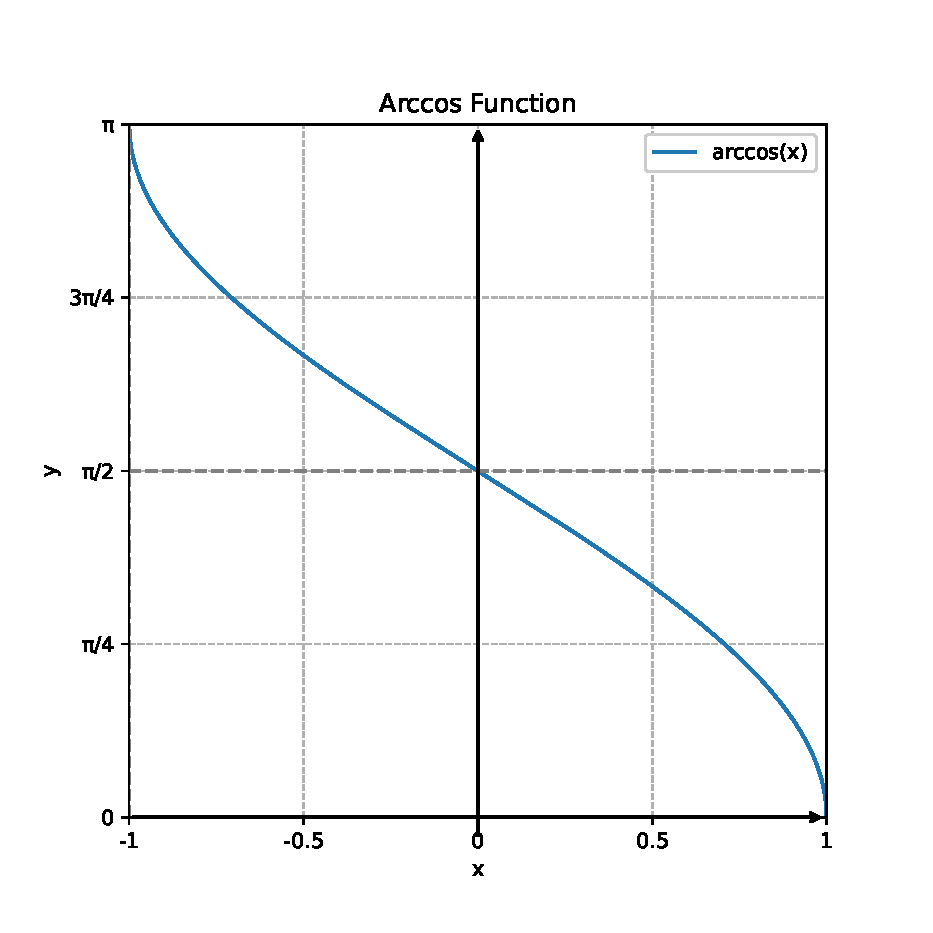
\includegraphics[width=0.4\columnwidth]{1.3.11.eps}
        }
        \caption{反正余弦函数图像}
    \end{figure}
    由于这两个函数分别是$\sin x$和 $\cos x$的反函数,因此可以知道的是,$\sin x$的值域是$\arcsin x$的定义域.因此可以得到下面的结论
    \begin{criterion}{反正余弦函数相关性质}{}
        \begin{itemize}
            \item 定义域$[-1,1]$,$y=\arcsin x$值域(主值区间)\footnote{描述一个函数所有值的区间}$[-\dfrac{\pi}{2},\dfrac{\pi}{2}]$,$y=\arccos x$值域(主值区间)$[0,\pi]$需要注意的是其值需要在值域内.因为只有在这个区间上,函数才满足反函数定义\ref{xxx1}中的唯一性.那么可以推断出如下的反函数:
            $$
            \text{当}x \in [-\frac{\pi}{2},\frac{\pi}{2}]\text{时},x=\arcsin y
            $$
            $$
            \text{当}x \in [\frac{\pi}{2},\frac{3\pi}{2}]时,x=\pi-\arcsin y
            $$
            $$
            \text{当}x \in [\frac{3\pi}{2},2\pi],x=2\pi+\arcsin y            
            $$
            \item 性质:$\arcsin x+\arccos x=\frac{\pi}{2}$(求导后可以发现导数为0)
        \end{itemize}
    \end{criterion}
    \begin{criterion}{反三角函数恒等式}{}
        $$
            \sin(\arcsin x)=x,x\in[-1,1],\sin(\arccos x)=\sqrt{1-x^2},x\in[-1,1];
        $$
        $$
            \cos(\arccos x)=x,x\in[-1,1],\cos(\arcsin x)=\sqrt{1-x^2},x\in[-1,1]\footnote{证明如下:令$t=\arccos x \in [0,\pi]$,$\cos t = x$,又$\sin ^2 t+\cos ^2 t=1$,那么$\sin t=\sqrt[2]{1-x^2}$,即$\sin(\arccos x)=\sqrt{1-x^2}$};
        $$
        上述两个式子可抽象为$f^{-1}f(x)=x$.
        除此之外,还有下面的等式
        $$
            \arcsin(\sin y)=y,y\in\left[-\frac{\pi}{2},\frac{\pi}{2}\right]
        $$
        $$
            \arccos(\cos y)=y,y\in\left[0,\pi\right]
        $$
    \end{criterion}
    \subsubsection{反正切和反余切函数}
    $$
        \boxed{y=\arctan x}
        \qquad \qquad \qquad \qquad \qquad \qquad
        \boxed{y=\arccot x}
    $$
    \begin{figure}[H] \centering
        \subfigure[反正切函数图像] {
            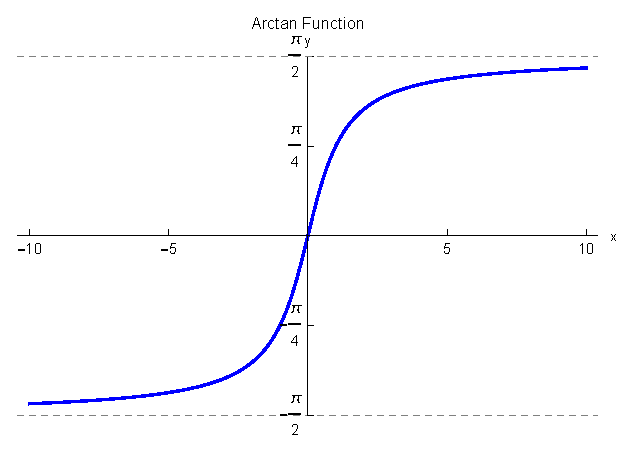
\includegraphics[width=0.4\columnwidth]{1.3.12.eps}
        }
        \subfigure[反余切函数图像] {
            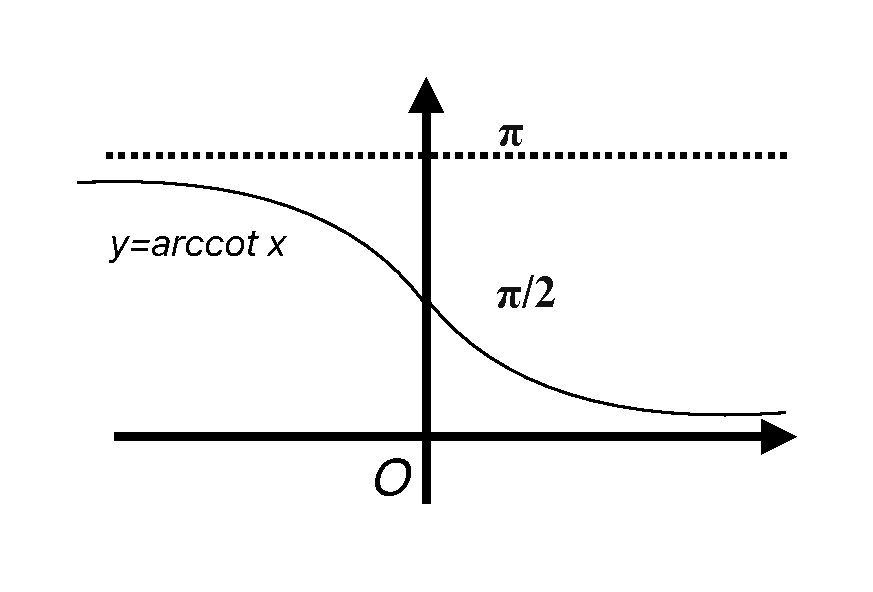
\includegraphics[width=0.45\columnwidth]{1.3.13.pdf}
        }
        \caption{反正余切函数图像}
    \end{figure}
    \begin{criterion}{反正余切函数相关性质}{}
        \begin{itemize}
            \item 定义域$[-\infty,+\infty]$,$y=\arctan x$值域$(-\frac{\pi}{2},\frac{\pi}{2})$,$y=\arccot x$值域$(0,\pi)$
            \item 性质:$\arctan x+\arccot x=\frac{\pi}{2}$(求导后可以发现导数为0)
        \end{itemize}
    \end{criterion}
    \subsection{初等函数}
    由基本初等函数经过有限次的四则运算,以及有限次的复合步骤所构成的并且可以由一个式子所
    表示的函数称为初等函数.
    \begin{criterion}{}{}
        幂指函数$u(x)^{\nu(x)}=e^{\nu(x)\ln u(x)}$也是初等函数,如$x>0$时,$f(x)=x^x=e^{x\ln x}$.其函数图像如下所示:
        \begin{figure}[H]
            \centering 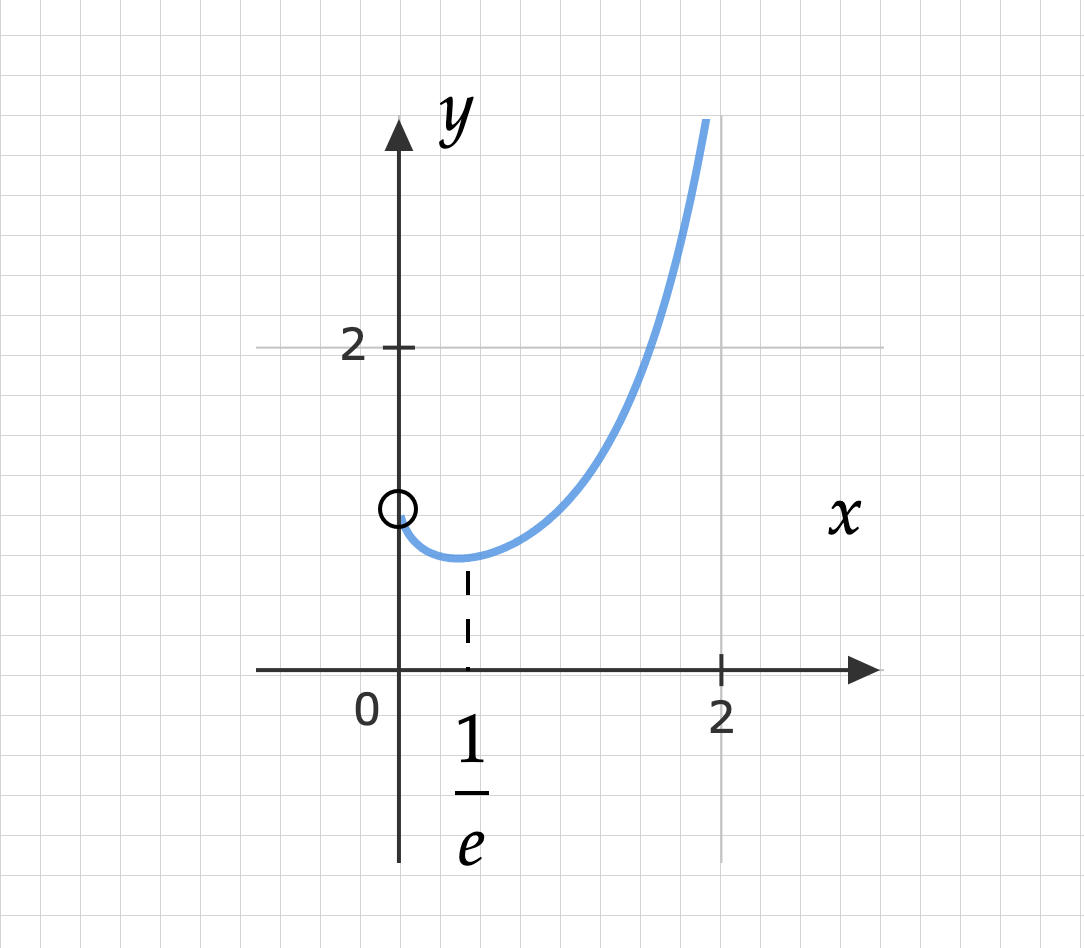
\includegraphics[width=
                0.3 \linewidth]{1.3.15.png} \caption{函数$x^x$图像}
        \end{figure}
    \end{criterion}
    \subsection{图像绘制}

    \subsubsection{极坐标下的图像}

    \begin{itemize}
        \item 用描点法绘制函数图像:就是把每一个点求出来,然后连接起来即可,但是需要点足够多
        \item 用直角坐标系观点画极坐标系的图像,以函数$r=2(1+\cos \theta )$为例.
              \begin{figure}[H]
                  \centering 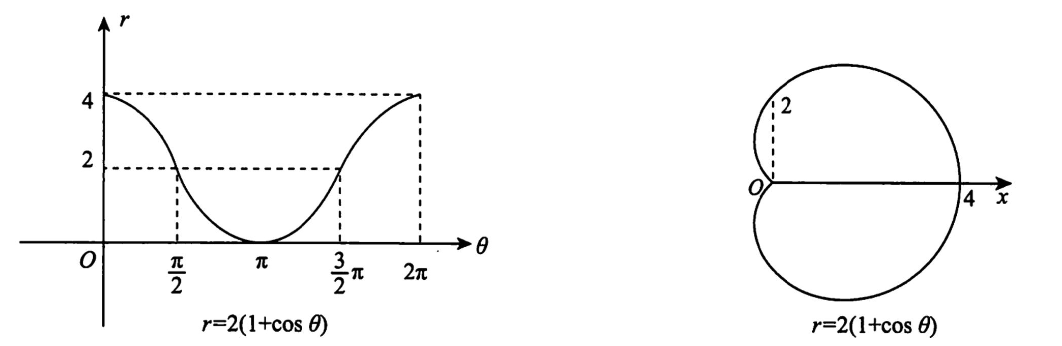
\includegraphics[width=
                      0.8 \linewidth]{1.3.14.png} \caption{函数$r=2(1+\cos \theta)$图像}
              \end{figure}
    \end{itemize}
    可以看到$\theta - r $的坐标系的关键点为$(0,4),(\frac{\pi}{2},2),(\pi,0),(\frac{3}{2}\pi,2),(2\pi,4)$这五个点,那么在极坐标系下可以绘制出这些点,比如在$x=4$时,$\theta = 0$,$x=2$时,$\theta = \frac{\pi}{2}$,$x=0$时,$\theta = \pi$.
    \subsubsection{参数方程}
    通过第三个变量即参数来表示别的两个变量.

    摆线参数方程:
    $$
        \left\{
        \begin{array}{l}
            x=r\left(t-\sin t\right) \\
            y=r\left(1-\cos t\right).
        \end{array}
        \right.
    $$

    星型线参数方程:
    $$
        \left\{
        \begin{array}{l}
            x=r \cos^3 t \\
            y=r \sin^3 t
        \end{array}
        \right.
    $$
    \section{常用函数知识}
    \subsection{三角函数}
    \subsubsection{三角函数基本关系}
    \begin{center}
        \boxed{
            \begin{aligned}
                 & \csc \alpha = \dfrac{1}{\sin \alpha} \quad \sec \alpha =\frac{1}{\cos \alpha} \quad \cot \alpha=\frac{1}{\tan \alpha} \\
                 & \tan \alpha = \dfrac{\sin \alpha}{\cos \alpha} \quad \cot \alpha=\frac{\cos \alpha}{\sin \alpha}
            \end{aligned}
        }
    \end{center}
    \subsubsection{倍角公式}
    \begin{center}
        \boxed{
            \begin{aligned}
                 & \sin2a=2\sin a\cos a,\quad\cos2a=\cos^2a-\sin^2a=1-2\sin^2a=2\cos^2a-1                              \\
                 & \sin3\alpha=-4\sin^3a+3\sin\alpha,\quad\cos3a=4\cos^3a-3\cos a                                      \\
                 & \tan2\alpha=\frac{2\tan\alpha}{1-\tan^2\alpha},\quad\cot2\alpha=\frac{\cot^2\alpha-1}{2\cot\alpha}.
            \end{aligned}
        }
    \end{center}
    \subsubsection{半角公式}
    \begin{center}
        \boxed{
            \begin{gathered}
                \sin^{2}\dfrac{\alpha}{2}=\frac{1}{2}\left(1-\cos\alpha\right),\quad\cos^{2}\frac{\alpha}{2}=\frac{1}{2}\left(1+\cos\alpha\right), \\
                \sin\dfrac\alpha2=\pm\sqrt{\frac{1-\cos\alpha}2},\quad\cos\frac\alpha2=\pm\sqrt{\frac{1+\cos\alpha}2}, \\
                \tan{\frac{\alpha}{2}}= \dfrac{1-\cos\alpha}{\sin\alpha}=\frac{\sin\alpha}{1+\cos\alpha}=\pm\sqrt{\frac{1-\cos\alpha}{1+\cos\alpha}}, \\
                \cot{\frac{\alpha}{2}}= \dfrac{\sin\alpha}{1-\cos\alpha}=\frac{1+\cos\alpha}{\sin\alpha}=\pm\sqrt{\frac{1+\cos\alpha}{1-\cos\alpha}}.
            \end{gathered}
        }
    \end{center}
    \subsubsection{和差公式}
    \begin{center}
        \boxed{
            \begin{aligned}
                 & \sin(\alpha\pm\beta)=\sin\alpha\cos\beta cos\alpha\sin\beta                  \\
                 & \cos(\alpha\pm\beta)=\cos\alpha\cos\beta\mp\sin\alpha\sin\beta               \\
                 & \tan(\alpha\pm\beta)=\dfrac{\tan\alpha\pm\tan\beta}{1\mp\tan\alpha\tan\beta}  \\
                 & \cot(\alpha\pm\beta)=\dfrac{\cot\alpha\cot\beta\mp1}{\cot\beta\pm\cot\alpha}.
            \end{aligned}
        }
    \end{center}
    \subsubsection{积化和差公式}
    \begin{center}
        \boxed{
            \begin{aligned}
                \sin\alpha\cos\beta= & \frac{1}{2}\big[\sin(\alpha+\beta)+\sin(\alpha-\beta)\big],\cos\alpha\sin\beta= & \frac{1}{2}\big[\sin(\alpha+\beta)-\sin(\alpha-\beta)\big], \\
                \cos\alpha\cos\beta= & \frac{1}{2}\big[\cos(\alpha+\beta)+\cos(\alpha-\beta)\big],\sin\alpha\sin\beta= & \frac{1}{2}\big[\cos(\alpha-\beta)-\cos(\alpha+\beta)\big].
            \end{aligned}
        }
    \end{center}
    \subsubsection{和差化积公式}
    \begin{center}
        \boxed{
            \begin{aligned}
                \sin\alpha+\sin\beta & =2\sin\frac{\alpha+\beta}{2}\cos\frac{\alpha-\beta}{2},\sin\alpha-\sin\beta=2\sin\frac{\alpha-\beta}{2}\cos\frac{\alpha+\beta}{2}   \\
                \cos\alpha+\cos\beta & =2\cos\frac{\alpha+\beta}{2}\cos\frac{\alpha-\beta}{2},\cos\alpha-\cos\beta=-2\sin\frac{\alpha+\beta}{2}\sin\frac{\alpha-\beta}{2}.
            \end{aligned}
        }
    \end{center}
    \subsubsection{万能公式}
    \begin{center}
        \boxed{
            \begin{aligned}
                \sin \alpha =\frac{2\tan \frac{\alpha}{2}}{1+\tan^2 \dfrac{\alpha}{2}} \\
                \\
                \cos \alpha=\frac{1- \tan^2 \frac{\alpha}{2}}{1+ \tan^2 \dfrac{\alpha}{2}}
            \end{aligned}
        }
    \end{center}
    \subsection{一元二次方程基础}
    \begin{itemize}
        \item 一元二次方程组:$a x^2 +bx+c=0(a \neq 0)$
        \item 根的公式:$x_{1,2}=\dfrac{-b\pm\sqrt{b^2-4ac}}{2a}$
        \item 根与系数的关系:$x_{1}+x_{2}=-\frac{b}{a},x_{1}x_{2}=\frac{c}{a}.$
        \item 判别式:$\Delta=b^2-4ac$
        \item 抛物线顶点坐标:$(-\dfrac{b}{2a},c-\dfrac{b^2}{4a})$
    \end{itemize}
    \subsection{因式分解公式}
    \begin{center}
        \boxed{
            \begin{aligned}
                 & (a+b)^2=a^2+2ab+b^2 \quad \quad (a-b)^2=a^2-2ab+b^2                                                            \\
                 & (a+b)^3=a^3+3a^2b+3ab^2+b^3 \quad \quad (a-b)^3=a^3-3a^2b+3ab^2-b^3                                            \\
                 & a^2-b^2=(a+b)(a-b) \quad \quad (a^3-b^3)=(a-b)(a^2+ab+b^2)                                                     \\
                 & a^3+b^3=(a+b)(a^2-ab+b^2)                                                                                      \\
                 & a^{n}-b^{n}=\left(a-b\right)\left(a^{n-1}+a^{n-2}b+\cdots+ab^{n-2}+b^{n-1}\right)\left(n\text{ 是正整数}\right)    \\
                 & n\text{ 是正奇数时 },a^{n}+b^{n}=\left(a+b\right)\left(a^{n-1}-a^{n-2}b+\cdots-ab^{n-2}+b^{n-1}\right)              \\
                 & (a+b)^n=\sum_{k=0}^n\text{C}_n^ka^{n-k}b^k=                                                                    \\
                 & a^n+na^{n-1}b+\frac{n(n-1)}{2!}a^{n-2}b^2+\cdots+\frac{n(n-1)\cdots(n-k+1)}{k!}a^{n-k}b^k+\cdots+nab^{n-1}+b^n \\
            \end{aligned}
        }
    \end{center}
    \subsection{阶乘与双阶乘}
    \begin{itemize}
        \item $n! =1\cdot2\cdot3\cdot\cdots\cdot n,\text{规定}0!=1.$
        \item $(2n)!!  =2\cdot4\cdot6\cdot\cdot\cdot(2n)=2^n\cdot n!$
        \item $(2n-1)!!  =1\cdot3\cdot5\cdot\cdot\cdot(2n-1)$
    \end{itemize}
    \subsection{绝对值等式}
    $$\varphi(x)=\operatorname*{max}\left\{f(x),g(x)\right\}=\frac{1}{2}[f(x)+g(x)+|f(x)-g(x)|]$$
    $$\quad\psi(x)=\operatorname*{min}\left\{f(x),g(x) \right\}=\frac{1}{2}[f(x)+g(x)-|f(x)-g(x)|]$$

    %  ############################
    \ifx\allfiles\undefined
\end{sloppypar}
\end{document}
\fi